%
% Template for Doctoral Theses at Uppsala 
% University. The template is based on    
% the layout and typography used for      
% dissertations in the Acta Universitatis 
% Upsaliensis series                      
% Ver 5.2 - 2012-08-08                  
% Latest version available at:            
%   http://ub.uu.se/thesistemplate            
%                                         
% Support: Wolmar Nyberg Akerstrom        
% Thesis Production           
% Uppsala University Library              
% avhandling@ub.uu.se                          
%                                         
%%%%%%%%%%%%%%%%%%%%%%%%%%%%%%%%%%%%%%%%%%%


\documentclass{UUThesisTemplate}

% Package to determine wether XeTeX is used
\usepackage{ifxetex}

\ifxetex
	% XeTeX specific packages and settings
	% Language, diacritics and hyphenation
	\usepackage[babelshorthands]{polyglossia}
	\setmainlanguage{english}
	\setotherlanguages{swedish}

	% Font settings
	\setmainfont{Times New Roman}
	\setromanfont{Times New Roman}
	\setsansfont{Arial}
	\setmonofont{Courier New}
\else
	% Plain LaTeX specific packages and settings
	% Language, diacritics and hyphenation
    % Use English and Swedish languages. 
	\usepackage[swedish,english]{babel} 

	% Font settings
	\usepackage{type1cm}
	\usepackage[latin1]{inputenc}
	\usepackage[T1]{fontenc}
	\usepackage{mathptmx}
	
	% Enable scaling of images on import
	\usepackage{graphicx}
	
	% Mathematical packages
	\usepackage{mathtools}
	\usepackage{amssymb}
	\usepackage{amsfonts}
% 	\usepackage[intlimits]{amsmath}
	\usepackage{bbm}
	\usepackage{braket}
	
	\usepackage{hyperref}
% 	\usepackage{slashed}
% 	\usepackage{psfrag}
% 	\usepackage{wasysym}
	\usepackage{esint}
	
% 	\usepackage[toc,page]{appendix}
\fi


% Tables
\usepackage{booktabs}
\usepackage{tabularx}

% Document links and bookmarks
\usepackage{hyperref} 

% Numbering of headings down to the subsection level
\numberingdepth{subsection}

% Including headings down to the subsection level in contents
\contentsdepth{subsection}


% Uncomment to use a custom abstract dummy text
\abstractdummy{
	\begin{abstract}
% 		Please use no more than 300 words and avoid mathematics or complex script.
	The gauge/string duality, a.k.a. the holographic principle is a profound assertion that emerged from string theory. 
	It relates strongly-coupled gauge theories to weakly coupled string theories living in a higher-dimensional curved geometry. 
	Nevertheless, it is a conjecture, and only a few instances of its more concrete form, the AdS/CFT correspondence, are well-understood. 
	The most well-studied example is the duality between N=4 SYM, which is a CFT, and type IIB string theory in AdS5xS5 background. 
	Generalization to less symmetric cases is a must, and the next logical step is to add a mass scale to N=4 SYM, 
	therefore breaking its conformal symmetry and leading to N=2* SYM, the theory we study in this thesis. 
	It is supersymmetric enough to employ the powerful localization method that reduces its partition function to a matrix model. 
	We will see that the mass scale causes non-trivial phase structures in its vacuum configuration, 
	visible in the holographic regime. We will probe them using Wilson loops in different representations of the gauge group. 
	On the other hand, the dual supergravity background was derived by Pilch-Warner, 
	making N=2* theory an explicitly testable non-conformal holographic case, which is a rare example. 
	We will prove that the duality works for the dual observables (string action, D-branes) we managed to compute, 
	even at a quantum-level. 	
	\end{abstract}
}


\begin{document}
\frontmatter
    % Creates the front matter (ti	tle page(s), abstract, list of papers)
    % for either a Comprehensive Summary or a Monograph.
    % Authors of Comprehensive Summaries use this front matter 
    \frontmatterCS 
    % Monograph authors use this front matter 
    %\frontmatterMonograph 
 
   % Optional dedication
%    \dedication{
% 	      He who has a why to live can bear almost any how. \\
%                --- \emph{Friedrich Nietzsche}
%                }
 
    % Environment used to create a list of papers
    \begin{listofpapers}
	\item
X.~Chen-Lin, J.~Gordon, and K.~Zarembo, ``{$ \mathcal{N}={2}^*$
  super-Yang-Mills theory at strong coupling},''
  \href{http://dx.doi.org/10.1007/JHEP11(2014)057}{{\em JHEP} {\bfseries 1411}
  (2014) 057},
\href{http://arxiv.org/abs/1408.6040}{{\ttfamily arXiv:1408.6040 [hep-th]}}.
	\item
X.~Chen-Lin and K.~Zarembo, ``{Higher Rank Wilson Loops in N = 2*
  Super-Yang-Mills Theory},''
  \href{http://dx.doi.org/10.1007/JHEP03(2015)147}{{\em JHEP} {\bfseries 1503}
  (2015) 147},
\href{http://arxiv.org/abs/1502.01942}{{\ttfamily arXiv:1502.01942 [hep-th]}}.	
	\item
X.~Chen-Lin, A.~Dekel, and K.~Zarembo, ``{Holographic Wilson loops in symmetric
  representations in $ \mathcal{N} = {2}^{\ast } $ super-Yang-Mills theory},''
  \href{http://dx.doi.org/10.1007/JHEP02(2016)109}{{\em JHEP} {\bfseries 02}
  (2016) 109},
\href{http://arxiv.org/abs/1512.06420}{{\ttfamily arXiv:1512.06420 [hep-th]}}.	
	\item
X.~Chen-Lin, ``{Symmetric Wilson Loops beyond leading order},''
  \href{http://dx.doi.org/10.21468/SciPostPhys.1.2.013}{{\em SciPost Phys.}
  {\bfseries 1} no.~2, (2016) 013},
\href{http://arxiv.org/abs/1610.02914}{{\ttfamily arXiv:1610.02914 [hep-th]}}.
    	\item 
X.~Chen-Lin, D.~Medina-Rincon, 	K.~Zarembo, ``{Quantum String Test of
  Nonconformal Holography},''
  \href{http://dx.doi.org/10.1007/JHEP04(2017)095}{{\em JHEP} {\bfseries 04}
  (2017) 095},
\href{http://arxiv.org/abs/1702.07954}{{\ttfamily arXiv:1702.07954 [hep-th]}}.
    	\label{apaperlabel}
    \end{listofpapers}
    
    
    \begingroup
        % To adjust the indentation in your table of contents, uncomment and enter the widest numbers for each level
        %  E.g.  \settocnumwidth{widest chapter number}{widest section number}{widest subsection number}...{...}
       %  \settocnumwidth{5}{4}{5}{3}{3}{3}
        \tableofcontents
    \endgroup
    
    % Optional tables
    %\listoftables
    %\listoffigures

\mainmatter
    
    % Include your chapters here.
    
    \chapter{Introduction}


The universe must be self-consistent. This is the basic premise physicists assume in the quest for the ultimate laws that govern our universe. Without it, a theory would be a mere description of a collection of observed facts. 

Despite highly precise experimental corroboration of the Standard Model of particle physics, which relies on Quantum Field Theory (QFT) with gauge symmetry, and Einstein's General Relativity (GR) that describes gravity, these two frameworks are mutually incompatible. That is without mentioning the foundational problems of QFT, that the Clay Mathematics Institute urges to solve with a million-dollar prize incentive\footnote{
See the link: \url{http://www.claymath.org/millennium-problems/yang\%E2\%80\%93mills-and-mass-gap} 
}.

Classical physics is elegantly formulated in terms of the least action principle. 
The standard procedure is to encode the dynamics in a quantity called action, 
minimize it with respect to the physical variables which gives a set of differential equations (of motion) to be solved. 
In quantum physics, we relax this principle. When quantizing a classical theory in Feynman path integral formulation, 
paths that do not minimize the action also contribute to the dynamics. In strong analogy with statistics, 
physical quantities are weighted observables $O$ by the exponential of the classical action\footnote{
The analogy is even closer when we analytically continue the time to pure imaginary time, i.e. Wick rotate $t \rightarrow -i t_{E}$, 
then the action becomes purely imaginary, and the exponential decays.}:
\[
 \braket{O} = \int D\phi \, O\, e^{-i S[\phi]/\hbar},
\]
where we used the shorthand notation $\phi$ for the collection of quantum fields\footnote{
Quantum mechanics can be formulated as a (0+1)-dimensional QFT.}. 
The problem is, however, the lack of a rigorous definition of the measure $D\phi$.
Very often, we only know how to compute quantum observables in certain limits, 
when we can rely on the saddle-point approximation to the integral. 
For example, in the classical limit (vanishing Plank constant $\hbar$), 
the saddle-point method for the partition function gives us the least action principle:
\[
 Z=\braket{1} \approx e^{-i S[\phi_c]/\hbar}; \quad  \delta S[\phi_c] = 0 .
\]
Other examples are the weak coupling limit, such as in Quantum Electrodynamics (QED), 
or the thermodynamic limit in quantum many-body systems. 
By contrast, we have no established analytical tool to handle strongly-coupled QFTs, 
which would explain quark confinement in Quantum Chromodynamics (QCD), and phases of high-Tc superconductors.

Only very few classes of path integrals are solvable. 
Besides free theories, path integrals of topological quantum field theories and some supersymmetric theories localize \emph{exactly} 
at their saddle-points. This highly non-trivial phenomenon is called the localization of path integrals, 
and it is one of the pillars our work is based on. 

Generalizing point-particles to strings, 
String Theory might be the best candidate for a consistent quantum gravity theory, 
which would be a unifying framework for QFT and GR. It is not free of mathematical problems though, 
for example the string action in a curved background is not fully known, 
and path integral measures are not rigorously defined either. Nevertheless, it is mathematically rich, 
with a web of dualities that connect different perturbative string theories (the underlying theory is known as the M-theory). 
It is offering us many insights otherwise unsuspected and a very important realization is the AdS/CFT correspondence. 
The most well-studied instance of the correspondence is the one between weakly-coupled superstring theory living on $AdS_5 \times S^5$ space, 
and a strongly-coupled supersymmetric conformal field theory (CFT) called $\mathcal{N}=4$  SYM. 
Despite much success (and still some issues concerning quantum stringy corrections), the correspondence remains an unproven conjecture.

An even more general correspondence is the gauge/string (or gauge/gravity) duality, 
also known as the holographic principle (so named because the gauge theory lives in a lower dimensional space than the string theory). 
If it were true, it would be revolutionary in many aspects. From a practical point of view,
on one hand we would have a toolbox to solve strongly-coupled gauge theories using essentially GR, 
and on the other hand, experiments on quantum gravity could be done in laboratories by handling systems like cold atoms. 
From a conceptual point of view, it could indicate that gravity, and hence spacetime, are emergent from lower dimensional quantum systems.

We lack the mathematical constructs to even formulate the conjecture in a precise manner. 
However, we can generalize what we learned from AdS/CFT to settings where we still hold some analytical control. 
A perfect toy model to investigate \emph{non-conformal} gauge/string duality is the unique massive deformation of $\mathcal{N}=4$ SYM, 
called $\mathcal{N}=2^*$ SYM.
On one hand, like $\mathcal{N}=4$ SYM, supersymmetric localization is applicable 
and reduces the complicated path integrals to a manageable matrix model,
allowing us to access its strongly-coupled regime (actually any finite coupling regime). 
On the other hand, $\mathcal{N}=2^*$ SYM 
is conjectured to be dual to a supergravity solution known as the Pilch-Warner background.
Figure \ref{fig:Overview} shows a graph on the relationship between different theories that we consider.
% Therefore, it is a golden opportunity to test the gauge/string duality beyond AdS/CFT, 
% and perhaps learn more about the string theory side through this duality. 


\begin{figure}[t]
\begin{center}
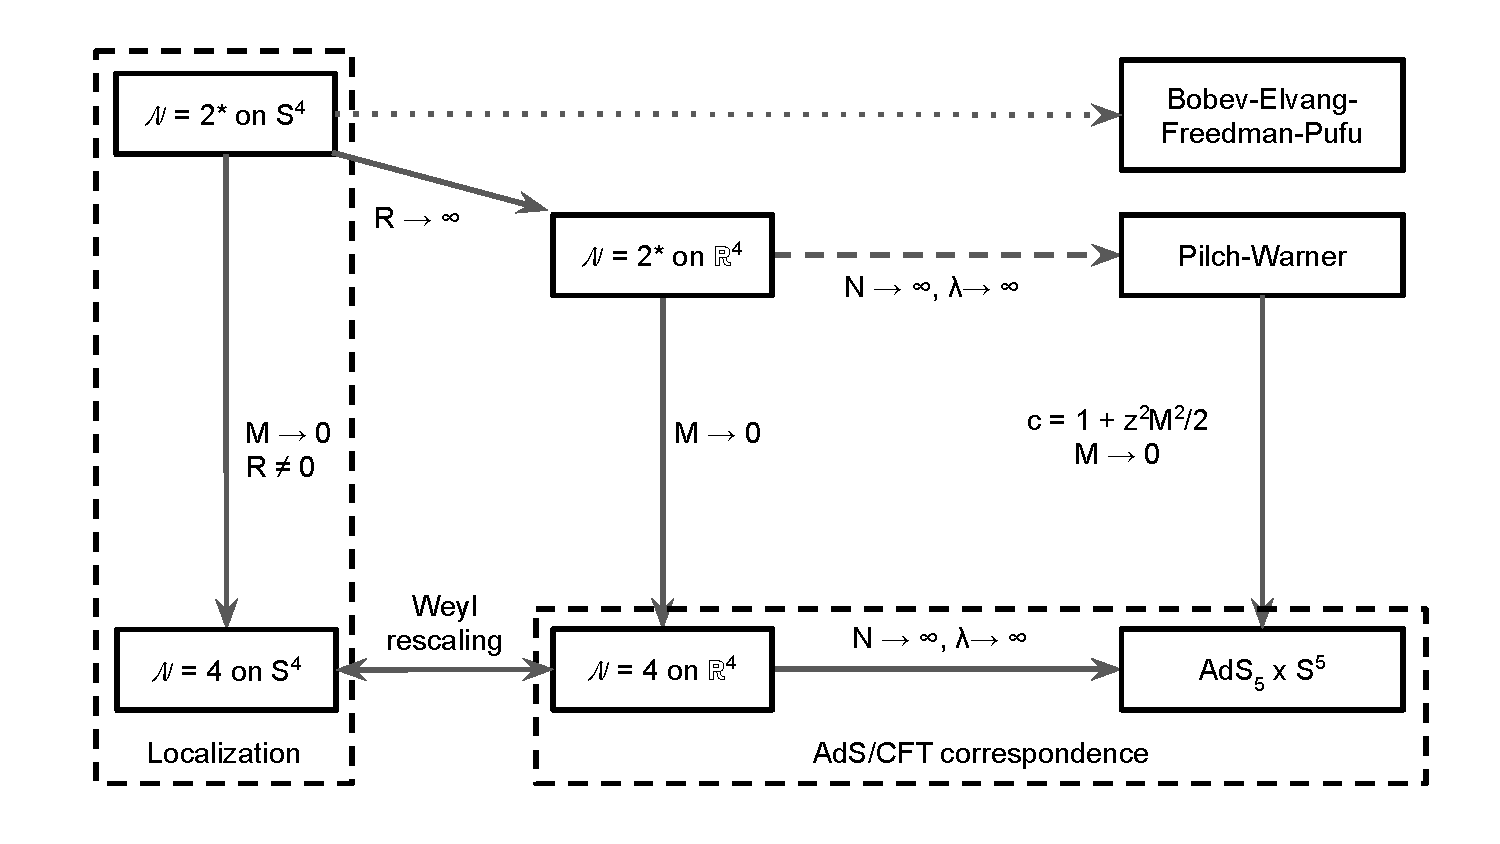
\includegraphics[width=\textwidth]{Images/Overview.pdf}
\end{center}
\caption{\label{fig:Overview} Localization applies to theories on the sphere, indicated by a dashed box. 
Since the gravity dual of $\mathcal{N}=2^*$ on $S^4$ is only partially known (indicated by the dotted line arrow), 
we take the decompactification limit ($R \rightarrow \infty$) to obtain $\mathcal{N}=2^*$ on $\mathbb{R}^4$.
Our research focuses on the dashed arrow,
which generalizes the well-established AdS/CFT correspondence shown in the dashed box below it. 
The limits will be explained through out the thesis.
%  in the 't Hooft limit ($N\rightarrow \infty$ and $\lambda \rightarrow \infty$), 
}
\end{figure}


\subsection*{Outline}
This thesis has two parts, both aimed at introducing and reviewing some background material in order to help the readers follow the appended papers.  
Part I focuses on the gauge theory side. We start off with the basics of the supersymmetric localization technique, 
then we go on to discuss the action of $\mathcal{N}=4$ SYM on $\mathbb{R}^4$ and on $S^4$. 
We then extend it to $\mathcal{N}=2^*$ SYM on $S^4$, and focus on the partition function after localization. 
We show the common technique to solve a matrix model, and conclude with the phase diagram of the theory. 
The last chapter of this part introduces the Wilson loop observables, and we review some known results in $\mathcal{N}=4$ case, 
and finally, write down the results we computed for $\mathcal{N}=2^*$ case. 
Part II starts with supergravity and some of its solutions, 
including $AdS_5\times S^5$ and Pilch-Warner. 
Then, we review the AdS/CFT correspondence and the logic behind its original derivation. In the end, we talk about holographic Wilson loops and connect our holographic solutions to the gauge theory results. 

\begin{quote}
 \emph{Physics is really nothing more than a search for ultimate simplicity, but so far all we have is a kind of elegant messiness.}
   ---  Bill Bryson
%  , \emph{A Short History of Nearly Everything}
\end{quote} 















   
   \part{Supersymmetric gauge theories }
     \chapter{Localization}
Localization of an integral happens when the integral is exactly equal to its saddle-point approximation.
% The localization loci are then the saddle-points.
A trivial example is therefore the Gaussian integration formula, which the saddle-point method is based on:
\begin{equation}\label{GaussianIntegral}
 \int_{\mathbb{R}^n} d^n x \, e^{-\frac{1}{2} x^T A x} = \sqrt{\dfrac{(2\pi)^n}{\text{det}A}},
\end{equation}
where $A$ is a positive-definite $n\times n$ matrix.


In the case of path integrals in quantum field theories, which are of infinite dimension,
localization, if applicable, reduces them to finite dimensional integrals.
% This is achieved using functional generalizations of the Gaussian formula \eqref{GaussianIntegral},
% and the resulting integral is over the moduli space of the theory vacua.
This is an exact approach, in contrast to perturbative methods such as Feynman diagrams,
valid only in the weakly-coupled regime.
Unfortunately, very few path integrals are solvable, 
but there are very specific classes of theories where localization does apply.
These are supersymmetric theories and topological quantum field theories,
from which we distinguish two types of localization:
supersymmetric localization and equivariant localization.
% As a matter of language, and
% this effect is often said to be \emph{semiclassically-exact}, or \emph{1-loop exact}.

Many results of this thesis are based on the supersymmetric localization.
We will review its basic idea and illustrate it explicitly in an example with an ordinary integral. 
We refer the reader to \cite{Szabo:1996md} and \cite{Pestun:2016zxk} for reviews of the topic.


\section{Supersymmetric localization}

In the path integral formulation of quantum theories, 
physical observables are expectation values of operators.
Let us consider the path integral (in the Euclidean signature and set $\hbar = 1$):
\begin{equation}
 \braket{O} = \int D\phi O \, e^{-S[\phi]},
\end{equation}
where $O$ is an operator, built out of the fields of the theory, represented by $\phi$.

Assume we can deform the action $S$ in such a way that it does not affect the physical quantity, 
namely
\begin{equation}
 \braket{O}_t = \int D\phi e^{-S[\phi]-t Q V[\phi]}, 
\end{equation}
where 
% $QV\geq 0$, and 
$Q$ is a fermionic symmetry of the theory, and require
\begin{equation}
 \dfrac{d \braket{O}_t}{d t} = 0.
%  \overset{!}{=} 0.
\end{equation}
Integrating by parts and assuming vanishing boundary terms, 
we obtain the following necessary conditions:
\begin{equation}\label{loc:susyCondition}
 Q^2 = 0, \quad Q S = 0, \quad Q O = 0,
\end{equation}
and that the measure $D\phi$ is also invariant (the symmetry must not be anomalous).

If this deformation were possible, then the deformation parameter $t$ could be of any value. 
The most useful case is to take it to be infinitely large,
in order to use the saddle-point approximation.
Since by construction the integral is independent of $t$, the saddle-point approximation must be exact,
hence the path integral localizes to a set of loci.
These are determined by\footnote{ 
If the bosonic part is positive-definite.
The fermionic contribution of the localization action is subleading.}
\begin{equation}\label{loc:saddlePoint}
 (QV)_\text{Bosonic} = 0
\end{equation}
whose solutions---let us denote them by $\phi_*$---belong to the moduli space of vacua of the theory.
This means that some fields acquire a non-zero vacuum expectation value.
Accounting the fluctuations around the vacuum configuration,
the localized integral can be formally written as:
\begin{equation}
 \braket{O}=\int_\text{Moduli} D\phi_* O(\phi_*) e^{-S(\phi_*)} Z_\text{1-loop},
\end{equation}
where the integral over $\phi_*$ is analogous to the sum over all the saddle-points, 
and $Z_\text{1-loop}$  is the functional generalization of the Gaussian integral \eqref{GaussianIntegral} for the fluctuations around the saddle-points. 
It is thus a functional determinant, which is divergent in general.
In order to obtain a finite result, the theory is defined in a compact manifold, like a sphere, 
such that the spectrum of the operator is discrete, and supersymmetry guarantees the cancellation of divergences between bosons and fermions.
Despite conceptual simplicity, the main challenge of this technique is to find the localization action $QV$, since no general recipe exists. 



\section{A toy example}

Consider an ordinary integral
\begin{equation}
 I = \int_m^M dx \,p g'(x)\,e^{p g(x)}, 
\end{equation}
with $p$ being a constant.
It can be solved exactly as a total derivative:
\begin{equation}
 I = \int_m^M  dx \, \dfrac{d}{d x}\,e^{p g(x)} 
   = e^{p g(M)}-e^{p g(m)}.
\end{equation}


If we were to solve it using the saddle-point approximation for $p \rightarrow \infty$,
then the saddle-points must be the endpoints $x_* = \{m, M\}$.
Let us consider this case and expand around the saddle-points:
\begin{equation}
 g(x_*+\xi) = g(x_*)+\frac{1}{2} g''(x_*) \xi^2 +\mathcal{O}(\xi^3).
\end{equation}
Each saddle-point contributes to the integral as following:
\begin{eqnarray}
 I_m &=& e^{p g(m)} \int_0^\infty  d\xi \, p g''(m) \xi\, e^{p \frac{1}{2} g''(m) \xi^2 } 
      =- e^{p g(m)} \\
 I_M &=& e^{p g(M)} \int_{-\infty}^0 d\xi \, p g''(M) \xi\, e^{p\frac{1}{2} g''(M) \xi^2 } 
      = e^{p g(M)}   
\end{eqnarray}
valid for $\Re(p g'') < 0$.
The sum $I_m + I_M$ indeed gives the exact result.
% In conclusion, the integral $I$ is a trivial example of localization.


Now, let us see how we can use supersymmetric localization to solve it. 
The integral $I$ can be rewritten in the supersymmetric form:
\begin{equation}
 I = \int_m^M \, dx \int da \int db \, e^{p(g(x)- a b g'(x))},
\end{equation}
where $a$ and $b$ are Grassmann numbers (our fermions), 
which means they satisfy $a b = -b a$ and $a^2=b^2=0$, hence 
\begin{equation} \label{GrassmannIntegral}
 f(x) = \int da \int db \, e^{-a\, f(x) \,b }.
\end{equation}


The action $S=p(g(x)-a b g'(x))$ is invariant under the supersymmetry transformation:
\begin{equation}
 \delta_\epsilon x = -\epsilon a, 
 \quad
 \delta_\epsilon a = 0,
 \quad 
 \delta_\epsilon b = \epsilon,
\end{equation}
where $\epsilon$ is a Grassmann number.
The supersymmetric operator, defined by $\epsilon Q = \delta_\epsilon$,
is explicitly
\begin{equation}
 Q = -a \frac{\partial }{\partial x}+\frac{\partial }{\partial b}.
\end{equation}
We can check that, indeed, \eqref{loc:susyCondition} are fulfilled.


Let us deform the integral with a $Q$-exact term
\begin{equation}
 I(t)=\int_m^M \, dx \int da \int db \, e^{p(g(x)-a b g'(x))+ t Q V},
\end{equation}
where 
\begin{equation}
 V(x, a, b) = f(x) b
\end{equation}
that leads to a non-trivial localization action
\begin{equation}
 QV = f(x)-a b f'(x).
\end{equation}
This is actually the most general supersymmetric action we can write for this case.
Thus, $S$ is not just $Q$-closed (i.e. $QS=0$), but also $Q$-exact (i.e. $S=QV_s$).


We require the deformed integral to be independent of the deformation parameter $t$:
\begin{equation}
 I'(t)=0.
\end{equation}
An explicit and straightforward computation shows
\begin{eqnarray}
 I'(t) &=& \int_m^M \, dx \int da \int db \, e^{S + t Q V} Q V \\
       &=& \int_m^M \, dx \int da \int db \, Q (e^{S + t Q V} V)\\
       &=& \left. e^{p g(x)+ t f(x)} f(x) \right|^M_m
\end{eqnarray}
where we used the supersymmetry condition and nilpotency. 
In this case, we must additionally require vanishing boundary conditions
\begin{equation}
 f(m)=f(M)=0.
\end{equation}

Now we can take large $t$ to solve the integral using the saddle-point method.
The boundary points here must be either global maxima or global minima of $f(x)$,
for $t>0$ or $t<0$, in order for the saddle-point integral to be convergent.
In other words, for $t$ negative (positive), 
the bosonic part of the localization action is positive (negative) definite, 
and it vanishes at the saddle-points:
\begin{equation}
 (QV)_\text{Bosonic}=0.
\end{equation}

The saddle-point approximation is exact, in the same fashion as for the large $p$ case we studied before.
This is to be expected, 
since the deformed integral is still a total derivative when we integrate out the fermions:
\begin{equation}
 I(t) = \int_m^M  dx \, \dfrac{d}{d x}\,e^{p g(x) + t f(x)} 
      = e^{p g(M)+ t f(M)}-e^{p g(m)+ t f(m)}.
%       = e^{p g(M)}-e^{p g(m)}.      
\end{equation}

When $g(x)=\cos x$ and the integration region is extended to a sphere 
parametrized by the polar angle $ x\in [0,\pi]$ and the azimuthal angle $\varphi \in [0, 2\pi]$,
this becomes a particular example of the Duistermaat-Heckman integration formula,
which is the precursor of the localization of path integrals.

% Witten used this example to illustrate the equivariant localization in the appendix of \cite{Witten:1992xu}.

% \begin{equation}
%   \int_0^{2\pi} d\phi \, \int_0^{\pi} \, d\theta \sin\theta \, e^{t \cos\theta}
% = \dfrac{2\pi}{t}\left(e^{t} - e^{-t}\right).
% \end{equation}
% The localization loci are the north and south pole, namely $\theta_*=\{0, \pi\}$.


% The theorem was later proved to be a special case of a more general localization property of equivariant cohomology
% and Berline and Vergne derived a localization formula for general compact Riemannian manifolds.
% The first infinite-dimensional generalization of the theorem,
% in the setting of a supersymmetric path integral,
% was worked out by Atiyah and Witten.



     \chapter{$\mathcal{N} = 4$ SYM}

Consider the action of a $d$-dimensional Yang-Mills (YM) theory 
with a massless spin-$\frac{1}{2}$ field $\Psi$ in the adjoint representation of the gauge group $U(N)$:
% (we will consider $SU(N)$)
\begin{equation}
 S = - \dfrac{1}{g_{YM}^2} \int d^d x \, \text{tr}
     \left(
         \dfrac{1}{2}F_{M N}F^{M N}
       - \bar{\Psi} \Gamma^M D_M \Psi 
     \right),    
\end{equation}
where $F_{M N} =\sum_{a=1}^{N^2} F_{M N}^a T^a_{ij}$, so that the trace is over the matrix indices $i, j=1, \ldots, N$. 
$T^a$ are the generators of the gauge group.
More explicitly, the field-strength and the covariant derivative are
\begin{eqnarray}
 F_{MN} &=& \partial_M A_N - \partial_N A_M + [A_M, A_N],\\
 D_M &=& \partial_M  + [A_M, \cdot],
\end{eqnarray}

% \begin{eqnarray}
%  F_{MN}^a &=& \partial_M A_N^a - \partial_N A_M^a + f_{abc} A_M^b A_N^c,\\
%  D_M \Psi^a &=& \partial_M \Psi^a + f_{abc} A_M^b \Psi^c,
% \end{eqnarray}
% where the structure constants $f_{abc}$ are defined by the commutation relation $[T^a, T^b]=f_{abc} T^c$.


In Minkowski spacetime $\mathbb{R}^{9,1}$, 
this action turns out to be invariant under the supersymmetry transformation:
\begin{eqnarray}
 \delta_\epsilon A_M  & = & \epsilon \Gamma_M \Psi,\\
 \delta_\epsilon \Psi & = & \dfrac{1}{2} F_{M N} \Gamma^{M N} \epsilon,
\end{eqnarray}
where $\epsilon$ is a constant Majorana-Weyl spinor that parametrizes the transformation.
% The bosonic and the fermionic degrees of freedom indeed match,
% \begin{itemize}
%  \item Bosonic: $D-2 = 8$
%  \item Fermionic: $2^{D/2}/2/2 = 8$
% \end{itemize}
% which is a necessary condition for supersymmetry. 

 
Lower dimensional supersymmetric theories can actually be obtained by 
dimensional reduction from the above theory \cite{Brink:1976bc}. 
Let us review how we can derive the action for the maximally supersymmetric
$\mathcal{N}=4$ SYM on $\mathbb{R}^{4}$.

\section{Action on $\mathbb{R}^{4}$}
The dimensional reduction consists of restricting the dependence of the fields only to 4 dimensions: $(x_1, \ldots, x_4)$.
The original Lorentz symmetry group $Spin(9,1)$ is then broken to $Spin(4) \times Spin(5,1)^R$,
that is the Lorentz group in 4d and an internal symmetry group called R-symmetry (hence the superindex $R$).
These groups are isomorphic to:
\begin{eqnarray}
Spin(4)      &=& SU(2)_L \times SU(2)_R \\
Spin(5, 1)^R &=& Spin(4)^R \times SO(1,1)^R \\
	     &=& SU(2)^R_L \times SU(2)^R_R \times SO(1,1)^R.
\end{eqnarray}
% where the subindexes $L, R$ refers to left and right. 

The gauge field $A_M$ is reduced to the 4d gauge field and scalars:
\begin{eqnarray}
 Spin(4):     & \,& A_\mu, \quad \mu = 1, 2, 3, 4 \\
%  Spin(5,1)^R: & \,& \Phi_I, \quad I = 0, 5, 6, 7, 8, 9
 Spin(4)^R: & \,& \Phi_I, \quad I = 5, 6, 7, 8 \\
 SO(1,1)^R: & \,& \Phi_I, \quad I = 0, 9 
\end{eqnarray}
where we wrote down the group they transform under.

The fermionic field, which is a Majorana-Weyl spinor, 
can be decomposed to 4 Majorana spinors (each having 2 degrees of freedom):
\begin{equation}
 \Psi=\begin{bmatrix}
       \psi_L\\
       \chi_R\\
       \psi_R\\
       \chi_L
      \end{bmatrix}
\end{equation}
where the spinors with the subindex $L$ (or $R$) transform in the spin-$\frac{1}{2}$ representation of
$SU(2)_L$ (or $SU(2)_R$).
Also, spinors with the name $\psi$ and $\chi$ transform in the spin-$\frac{1}{2}$ representation of
$SU(2)_L^R$ and $SU(2)_R^R$ from the R-symmetry subgroup, respectively.




The $\mathcal{N}=4$ SYM action explicitly written in terms of the 4d bosonic fields is:
\begin{equation}\label{SR4}
  \begin{split}
    S_{\mathbb{R}^4} = - \dfrac{1}{g_{YM}^2} \int d^4 x \, \text{tr}
    (
         \dfrac{1}{2}F_{\mu \nu}F^{\mu \nu}
       + D_\mu \Phi_I D^\mu \Phi^I
       + \dfrac{1}{2} [\Phi_I, \Phi_J]\, [\Phi^I, \Phi^J]       
    \\
       \qquad
       - \bar{\Psi} \Gamma^\mu D_\mu \Psi 
       - \bar{\Psi} \Gamma^I [ \Phi_I, \Psi ]
    ),
   \end{split}
\end{equation}
where we decomposed the 10d gamma matrices as $\Gamma^M=\Gamma^\mu \otimes \Gamma^I$.


The action has no mass scale, and it is in fact conformal invariant even at quantum level \cite{MANDELSTAM1983149, BRINK1983323}.
The conformal group extends the Poincar\'e group (translation, rotations and boosts) 
to include scaling (dilatation),
and special conformal transformation, which is a composition of inversion, translation and inversion.
The conformal symmetry, the four copies of supersymmetry and the internal R-symmetry
are part of the larger $\mathcal{N}=4$ superconformal group $PSU(2,2|4)$.
Its Lie algebra is generated by the generators of the conformal algebra, 
16 supercharges (that commute with momentum generators),
and 16 superconformal charges (that commute with special conformal generators). 
Details of the algebra can be found for example in \cite{Minahan:2010js}.


\section{Action on $S^4$}
In order to apply supersymmetric localization to $\mathcal{N}=4$ SYM, 
we shall put this theory on a hypersphere $S^4$.
% , which can be done using conformal invariance.
Conformal invariance implies an additional conformal coupling of the scalars to the scalar curvature $\mathcal{R}$, 
namely,
\begin{equation}\label{conformalCoupling}
 \dfrac{\mathcal{R}}{6} \Phi^I \Phi_I, \quad I=0,5,6,7,8,9
\end{equation}
where for $S^d$ with radius $R$, the scalar curvature is $\mathcal{R} = d(d-1)/R^2 $.
Then, there will be also a metric factor $\sqrt{g}$ coming from the curved background.
The action on $S^4$ is hence
\begin{equation}\label{SS4}
  \begin{split}
    S_{S^4} = - \dfrac{1}{g_{YM}^2} \int d^4 x \, \sqrt{g} \text{tr}
    \left(
        \dfrac{1}{2}F_{\mu \nu}F^{\mu \nu}
       + D_\mu \Phi_I D^\mu \Phi^I
       + \dfrac{1}{2} [\Phi_I, \Phi_J]\, [\Phi^I, \Phi^J]       
    \right. \\
    \left. 
       \qquad
       - \bar{\Psi} \Gamma^\mu D_\mu \Psi 
       - \bar{\Psi} \Gamma^I [ \Phi_I, \Psi ]
       + \dfrac{2}{R^2} \Phi^I \Phi_I
    \right).
   \end{split}
\end{equation}
Localization also requires the existence of an off-shell supersymmetry.
To fulfill this condition, additional auxiliary field terms are added to the above action, see \cite{Pestun:2007rz, Festuccia:2011ws}.
Then, on the localization locus, the action will effectively be $3/2$ times the conformal coupling \eqref{conformalCoupling}, 
see also \cite{Russo:2013qaa}.
Naturally, at the decompactification limit $R \rightarrow \infty$, we recover the flat space version.
% We shall see this limit is important for many of our results.







\chapter{$\mathcal{N} = 2^*$ SYM}

The fields of $\mathcal{N}=4$ SYM form a $\mathcal{N}=4$ vector (or gauge) multiplet, 
but the latter can be decomposed into two $\mathcal{N}=2$ massless supermultiplets, namely
\begin{eqnarray}
 \text{Vector multiplet:} & & \{A_1, A_2, A_3, A_4, \Phi_0, \Phi_9, \psi_L, \psi_R\},  \\
 \text{Matter hypermultiplet:} & &\{\Phi_5, \Phi_6, \Phi_7, \Phi_8, \chi_L, \chi_R\}.
\end{eqnarray}	

$\mathcal{N}=2^*$ SYM is the unique massive deformation of $\mathcal{N}=4$ SYM that breaks half of its supersymmetries.
This is achieved by giving mass to the matter hypermultiplet, 
either via the $\mathcal{N}=1$ superpotential \cite{Buchel:2000cn, Bobev:2013cja}, 
or using Scherk-Schwarz reduction of $\mathcal{N}=1$ SYM \cite{Pestun:2007rz, Scherk:1979zr}.
The latter prescribes the following replacement rules in the action \eqref{SR4}:
\begin{eqnarray}
D_0 \Phi_i &\rightarrow & D_0 \Phi_i + M_{ij} \Phi_j, \quad i,j =5,\ldots 8 \\
D_0 \chi &\rightarrow & D_0 \chi + \dfrac{1}{4}\Gamma_{ij} M_{ij} \chi,
\end{eqnarray}
where $M_{ij}$, a $4 \times 4$ matrix, is a generator of $SU(2)^R_R$,
and is normalized as $M_{ij} M^{ij} = 4 M^2$, where $M$ is the mass scale. All the repeated indices are summed over.
These replacements will give the standard mass term to the bosons and the fermions, 
and a cubic coupling term for the scalars. 
In its infinite-mass limit, the matter hypermultiplet can be integrated out, 
and the resulting theory is the pure $\mathcal{N}=2$ SYM.


% The full mass term to be added to the massless theory is:
% \begin{equation}
%  S_\text{mass} = \dfrac{1}{2 g_{YM}^2} \int d^4 x \, \sqrt{g} 
%  \text{tr} \left( m^2 \Phi_i \Phi^i + m (\chi_1 \chi_1 + \chi_2 \chi_2 + h.c.) 
%            -\dfrac{1}{4 r} R_{ki} M_{kj} \Phi^i \Phi^j
%            \right)
% \end{equation}
In order to apply the localization method to the partition function of $\mathcal{N}=2^*$ SYM,
we need to put it on $S^4$.
Since the theory is no longer conformal due to the hypermultiplet mass scale,
an additional curvature correction term to the mass is required in order to preserve supersymmetry, 
besides the conformal coupling discussed in \eqref{SS4}.
% Moreover, localization requires off-shell supersymmetry, and that is fixed by an auxiliary field term to the action.
The full action can be found in \cite{Pestun:2007rz}, with the details of the localization procedure therein.
We are interested in the final localized result, that we will discuss next.

% In the limit of infinitely heavy hypermultiplet, these fields possess no dynamic degrees of freedom,
% hence we can integrate them out and then the resulting theory is the pure $\mathcal{N}=2$ SYM. 



\section{Partition function}

Theories with an action can be quantized using a path integral.
The partition function in Euclidean signature is defined as
% \footnote{
% Wick rotation analytically continues time to imaginary (Euclidean) time, $t\rightarrow -i t_E$,
% then the oscillatory exponential becomes decaying. }
% the same as the canonical partition function in statistical mechanics. }
\begin{equation}
 Z = \int D\phi \, e^{-S[\phi]},
\end{equation}
which is an infinite-dimensional integral, 
over all possible field configurations (represented by the measure $D\phi$) on all of spacetime.


For $\mathcal{N}=2^*$ on $S^4$ and its limiting cases $\mathcal{N}=4$ (massless hypermultiplet) and pure $\mathcal{N}=2$ (infinitely-heavy hypermultiplet that is integrated out), 
there is one localization locus.
It is the moduli space of Coulomb vacua, 
parametrized by the vacuum expectation value of a scalar of the vector multiplet:
\begin{equation}\label{vevScalar}
 \braket{\Phi_0} = \text{diag}(a_1, \ldots, a_N), 
\end{equation}
where $a_i$ are real numbers.
The Coulomb phase of the theory 
is a consequence of the spontaneous symmetry breaking of the bosonic quartic potential $\sim [\Phi_I, \Phi_J]^2$,
that breaks the original gauge group $U(N)$ to $U(1)^{N}$.

The result for the localized partition function is of the form:
\begin{equation}\label{Zmatrixmodel}
 Z=\int \; d^N a \, \prod_{i<j} (a_i-a_j)^2 \; Z_\text{1-loop}(a)\; \left|Z_\text{inst}(a)\right|^2\; e^{- \frac{8\pi^2 N}{\lambda} \sum_k a_k^2}.
\end{equation}
The classical action comes from the curvature coupling of the scalars in \eqref{SS4}.

The 1-loop correction, for the different theories are
\begin{eqnarray}
 \text{$\mathcal{N}=2^*$ SYM:}  & & Z_\text{1-loop} = \prod_{i<j} \dfrac{H^2(a_i-a_j)}{H(a_i-a_j-MR) H(a_i-a_j+MR)}\\
 \text{$\mathcal{N}=2$ SYM:}  & & Z_\text{1-loop} = \prod_{i<j} H^2(a_i-a_j) \\
 \text{$\mathcal{N}=4$ SYM:}  & & Z_\text{1-loop} = 1
\end{eqnarray}
where 
\begin{equation}
 H(x) \equiv \prod_{n=1}^{\infty}\left(1+\dfrac{x^2}{n^2}\right)^n e^{-\frac{x^2}{n}}.
\end{equation}
% This function is $1$ at the origin and vanishes very fast away from it.
We used the 't Hooft coupling $\lambda = g_{YM}^2 N$,
and $R$ is again the radius of the hypersphere.


The instanton partition function is the generating function of instantons of topological charge $k$:
\begin{equation}
 Z_\text{inst} = \sum_{k=0}^\infty (e^{i 2\pi\tau})^k Z_k,
\end{equation}
where $Z_0 = 1$ and 
\begin{equation}
\tau = i \frac{4\pi}{g_\text{YM}^2} + \frac{\theta}{2\pi} 
\end{equation}
is the complexified Yang-Mills coupling\footnote{
The instanton action is the pure Yang-Mills action with an additional topological term.
For an instanton of charge $k$, the action is given by:
\[
S_\text{YM} (k)=
    -\frac{1}{2 g_\text{YM}^2} \text{tr} \int d^4 x \sqrt{g} F_{\mu\nu} F^{\mu\nu}
    -i \frac{\theta}{8\pi^2} \text{tr} \int F \wedge F 
    = \left( \frac{8\pi^2}{g_\text{YM}^2} - i \theta \right) k
    = - i 2 \pi \tau \, k. 
\]
% This action breaks CP symmetry.
% In QCD, there is no experimental evidence of CP violation, hence $\theta$ must be very small,
% and it is a considered a fine-tuning problem called the strong CP problem.
}.
% Instantons are tunnelling events in Minkowski signature
% In QCD, the groundstate, called the $\theta$-vacuum, is considered the superposition of all vacua. }.

For the $\mathcal{N}=4$ case, $Z_\text{inst} = 1$, \cite{Okuda:2010ke}.
For the $\mathcal{N}=2$ cases, it is non-trivial, \cite{Nekrasov:2002qd}.
However, the regime of interest is the large $N$ limit:
\begin{equation}\label{largeNlimit}
 N\rightarrow \infty \quad \text{and} \quad \lambda = g_\text{YM}^2 N \quad \text{is kept finite},
\end{equation}
then the expansion parameter becomes
$$e^{i 2\pi\tau}=e^{-\frac{8\pi^2 N}{\lambda} + i \theta},$$
hence the instanton contributions are expected to be exponentially suppressed. 
This is checked in \cite{Russo:2013kea}.


% 
% for a single instanton in $\mathcal{N}=2^*$
% \begin{equation}
%  Z_\text{1-inst} = - e^{-\frac{8\pi^2 N}{\lambda} + i \theta} (M R)^2 
% 		  \sum_{l=1}^N \prod_{j\neq l}^N \dfrac{ (a_l-a_j +i)^2 - (MR)^2}{(a_l-a_j) (a_l-a_j+2i)}
% \end{equation}
% Integral representation
% \begin{equation}
%  Z_\text{1-inst} = e^{-\frac{8\pi^2 N}{\lambda} + i \theta} \dfrac{2 (M R)^2}{(M R)^2+1} 
% 		  \int \frac{dz}{2\pi} \prod_{j=1}^N \dfrac{(z-a_j)^2 - (MR)^2}{(z-a_j)^2+1}
% \end{equation}









\section{Large-$N$ matrix model}

The localized partition function \eqref{Zmatrixmodel} is a matrix model.
% Therefore, it is convenient to think of it as an analogous statistical model, as we shall see.
For the $\mathcal{N}=4$ case, the model is particularly simple, 
it is the well-known Gaussian unitary ensemble (GUE) in the random matrix theory.
The product of the eigenvalue differences is the Vandermonde determinant squared, 
which is essentially the Jacobian factor after diagonalizing the Hermitean matrix in \eqref{vevScalar}.
Writing it in terms of the effective action:
\begin{equation}\label{eq:ZGUE}
 Z_\text{GUE} = \int \; d^N a \;  e^{- S[a]}, 
 \quad S[a]=- \sum_{i\neq j}^N \log(|a_i-a_j|) + \frac{8\pi^2 N}{\lambda} \sum^N_k a_k^2
\end{equation}
we see that the Vandermonde determinant gives the 2d Coulomb potential.
This partition function is indeed identified with that of a 2d Coulomb gas confined on a line,
with the repulsive electrostatic force and an attractive harmonic force \cite{Dyson:1962es}.


% Exact methods exist, 
% such as the orthogonal polynomial method, 
% to solve the spectral distribution.
% These allow physicists to compute observables exactly for $\mathcal{N}=4$ (cite Genis).

For $\mathcal{N}=2^*$, the matrix model is highly non-trivial, 
but we can solve it systematically in the large $N$ limit,
where the saddle-point approximation and the continuous approximation in principle apply.
The only relevant quantity to compute then is the distribution of the eigenvalues:
\begin{equation} \label{def:rho}
\rho(x) = \dfrac{1}{N} \, \sum_{i=1}^N \delta(x-a_i) .
\end{equation}
It must have a compact support, i.e. $\rho(\pm \mu) = 0$,
where the endpoint $\mu$ determines the scale of the spontaneous symmetry breaking.
By definition, it is also unit-normalized:
\begin{equation}
 \int_{-\mu}^\mu dx\, \rho(x) = 1.
\end{equation}


The saddle-point equation, from extremizing the effective action \eqref{eq:ZGUE} in terms of \eqref{def:rho}, 
is a singular (principal value) integral equation:
\begin{equation} \label{saddlepointEq}
 \dfrac{\delta S [\rho]}{\delta \rho(x)} = 0 \quad
 \Rightarrow \quad
 \fint_{-\mu}^\mu dy \, K(x-y) \rho(y) = \dfrac{8\pi^2}{\lambda}x.
\end{equation}
The singular kernel for the GUE case is just the Hilbert kernel\footnote{
The name is in relation with the Hilbert transform. 
It is also known as Cauchy kernel in the literature.},
that is 
\begin{equation}
 K_\text{Hilbert}(x)=\dfrac{1}{x}.
\end{equation}
In the Coulomb gas picture, the saddle-point equation determines the equilibrium distribution due to the force balance.
The result is the well-known Wigner's semicircle distribution
\begin{equation}\label{semicircle}
 \rho(x) = \dfrac{2}{\pi \mu^2} \sqrt{\mu^2-x^2}, 
 \quad \mu = \dfrac{\sqrt{\lambda}}{2\pi},
\end{equation}
shown in figure \ref{fig:semicircle}.


\begin{figure}[t]
\begin{center}
 \centerline{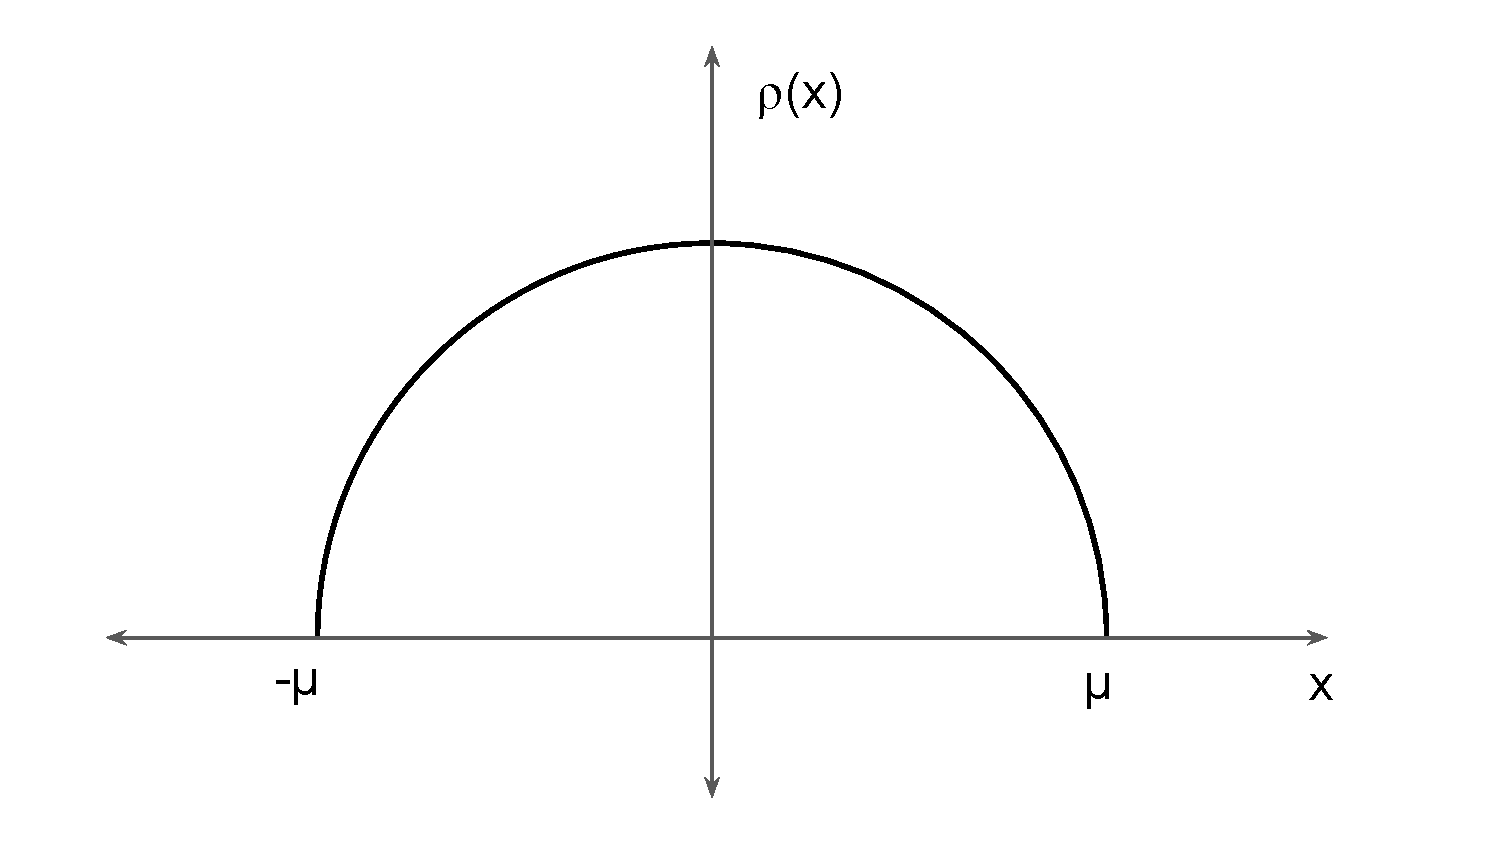
\includegraphics[width=0.8\textwidth]{Images/semicircle.pdf}}
 \caption{\label{fig:semicircle} Wigner's semicircle distribution, solution to the Gaussian unitary ensemble (GUE).}
\end{center}
\end{figure}

For the $\mathcal{N}=2^*$ SYM, the kernel is
\begin{equation}
 K(x)=\dfrac{1}{x}-\mathcal{K}(x)+\dfrac{1}{2}\,\mathcal{K}(x+MR)+\dfrac{1}{2}\,\mathcal{K}(x-MR),
\end{equation}
where 
\begin{equation}
 \mathcal{K}(x) \equiv -\dfrac{H'(x)}{H(x)} 
                = 2x\sum_{n=1}^{\infty} \left(\dfrac{1}{n}-\dfrac{n}{n^2+x^2} \right),
\end{equation}
and much more interesting features show up in the saddle-point solution, as shown in figure \ref{fig:phaseDiagram}.
Let us briefly review these results.


In the strong-coupling regime, the bulk of the distribution is also a semicircle but with a rescaled endpoint:
\begin{equation}\label{semicircleN=2*}
 \rho(x) = \dfrac{2}{\pi \mu^2} \sqrt{\mu^2-x^2}, 
 \quad
 \mu=\dfrac{\sqrt{\lambda (1+(MR)^2)}}{2\pi},
 \quad (\lambda \rightarrow \infty).
\end{equation}
This is due to the fact that the kernel is approximately a Hilbert kernel \cite{Buchel:2013id}:
\begin{equation} \label{Kapprox}
 K(x) \approx \dfrac{1+(MR)^2}{x}, \quad (\lambda \rightarrow \infty).
\end{equation}
Close to the edge-points, this approximation no longer holds,
and it was the goal of Paper I to find the endpoint distribution in the strong coupling regime.

We computed the endpoint distribution exactly using the so-called Wiener-Hopf method, 
which is essentially the Fourier transform of the convolution integral in \eqref{saddlepointEq} in a semi-infinite interval 
(zero being at the endpoint),
that relies on a certain factorization of the kernel.

The distribution exhibits oscillatory behavior with a period proportional to the scale $M R$. 
In the decompactification limit $MR\rightarrow \infty$ (but $\mu\gg MR$ because we remain in the strong coupling limit), 
the peaks of the oscillation diverge, see figure \ref{fig:phaseDiagram}.
The analytical endpoint distribution at strictly infinite coupling and flat space, with $\xi\equiv\mu-x$, is summarized below:
\begin{equation}
 \rho(\xi )= \frac{2^{3/2}}{\pi \mu^{3/2}}
% \frac{\sqrt{2 M R}}{\pi \mu^{3/2}}
 \begin{cases}
   MR \sqrt{\xi}, 
   &\quad (\xi \sim 1)\\
   \dfrac{\sqrt{M R}}{2}\sum_{k=0}^{\left[\frac{\xi }{MR}\right]}
             \left(\left\{\frac{\xi }{MR}\right\} + k\right)^{-1/2}
   &\quad (\xi \sim M R),
 \end{cases}
\end{equation}
where $[\cdot]$ and $\{\cdot\}$ denote the integer and the fractional part, respectively, 
and $\mu=MR\sqrt{\lambda}/(2\pi)$, from \eqref{semicircleN=2*}.

Physically, the cusps appear due to a resonance phenomena 
\begin{equation}
m_{ij} = |a_i-a_j \pm MR| \approx 0
\end{equation}
of very light states in the hypermultiplet sector.
Similar features were already observed for finite couplings in the flat space limit \cite{Russo:2013qaa},
and it was numerically shown that there are infinite-many critical couplings defined by 
\begin{equation}
 \mu = g(\lambda_c^{(n)}) M R, \quad g(\lambda_c^{(n)}) = \dfrac{n}{2}, \quad n=1,\ldots
\end{equation}
This means there are infinitely many phase transitions, where the phases are distinguished by the number of cusps of the distribution,
and the coupling $\lambda$ is the order parameter.
At strong coupling, the critical behavior persists and matches with the one obtained from the decompactification limit, 
hence these two limits commute \cite{Zarembo:2014ooa}.




\begin{figure}[t]
\begin{center}
 \centerline{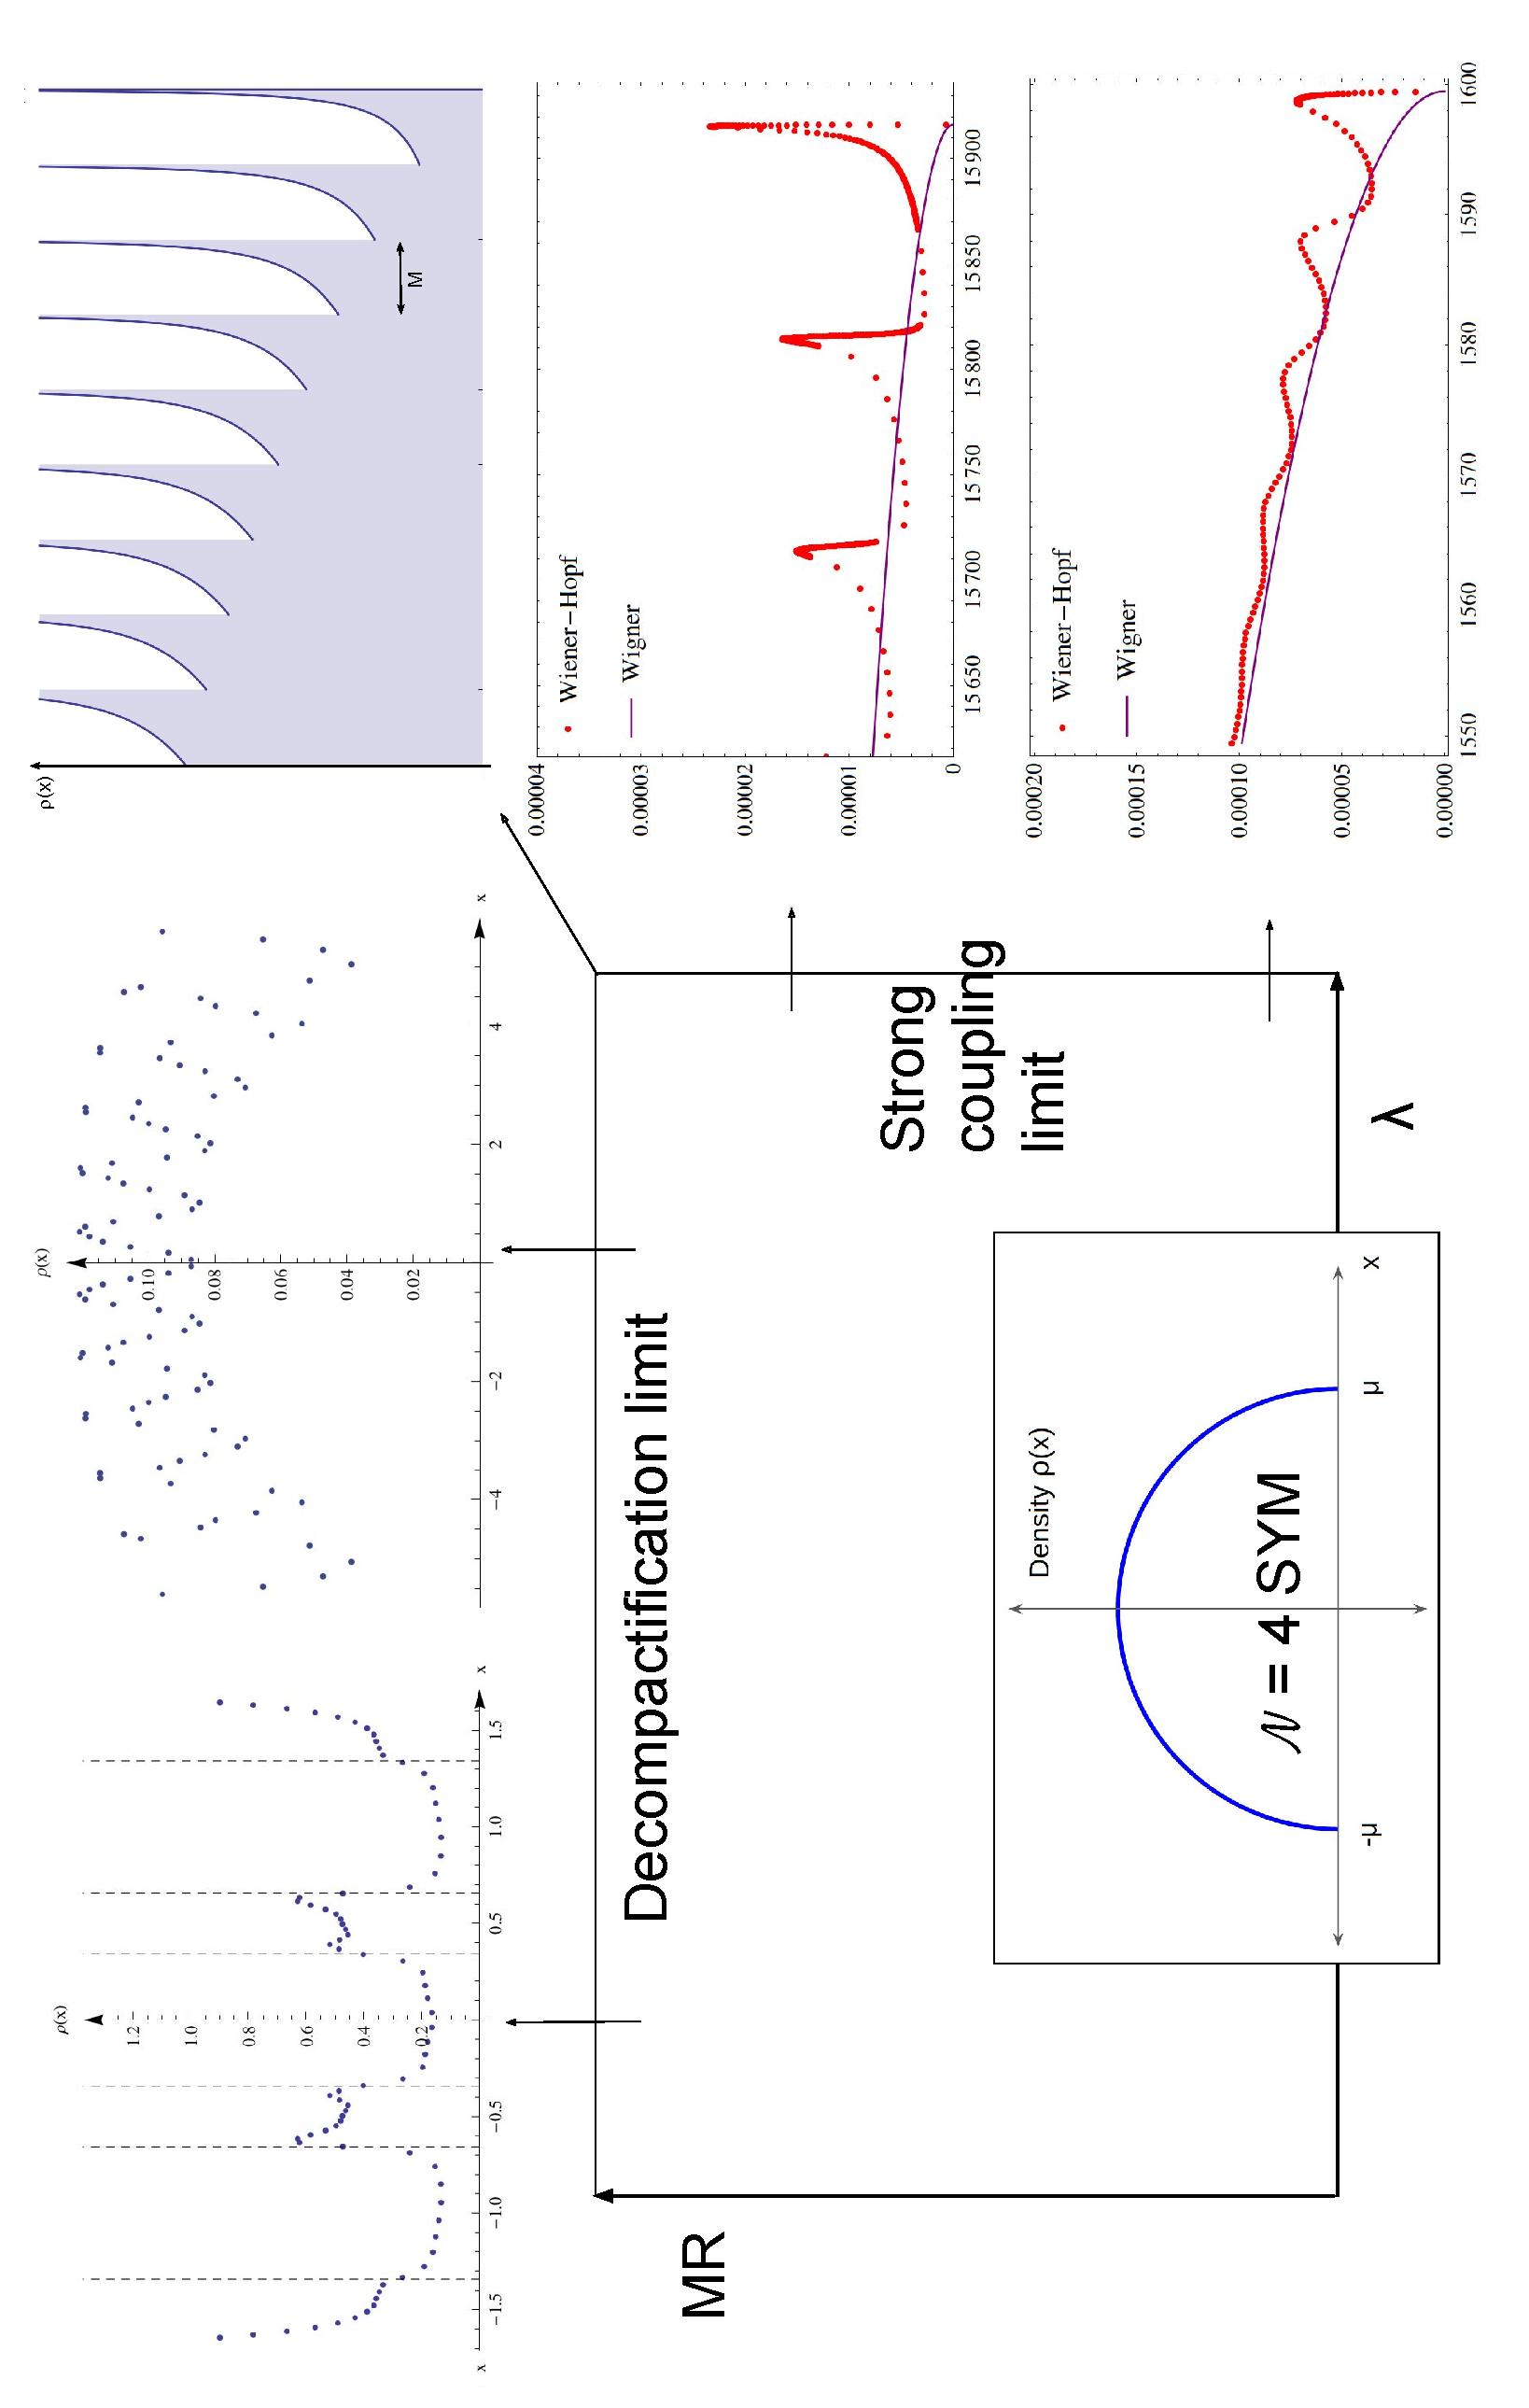
\includegraphics[width=0.9\textwidth]{Images/phaseDiagram.pdf}}
\end{center}
\caption{\label{fig:phaseDiagram} Phase diagram for the partition function of $\mathcal{N}=2^*$ SYM on $S^4$, in the large $N$ limit. 
The plots at the decompactification limit are taken from \cite{Russo:2013qaa}, and the ones at strong coupling limit are from Paper I, where only close to the endpoint is shown and $R=1$.
In the zero mass limit, we have $\mathcal{N}=4$ SYM, where the distribution is the Wigner semicircle for any coupling.}
\end{figure}


Such phase transitions are common among large-$N$ matrix models, 
and have been observed in e.g. ABJM models \cite{Anderson:2014hxa}, 5d $\mathcal{N}=1$ SYM with massive matter multiplets \cite{Nedelin:2015mta}.
In our case, the gauge/string duality in principle gives us an opportunity to understand them from the point of view of gravity.
The physical observables we use to probe the infinite-coupling phase are Wilson loops, the topic of the next chapter.








% \section{Action }

% Let us first review how to obtain the actions of our theories. 
% We will start with the action of $\mathcal{N}=4$ SYM on $\mathbb{R}^{3,1}$. 
% It is convenient to use the language of $\mathcal{N}=1$ SYM in $\mathbb{R}^{9,1}$, 
% from which all supersymmetric actions for lower dimensional Yang-Mills theory can be obtained from (cite someone).
% 
% The action is 
% \begin{equation}
%  S = \int d^4 x\, \sqrt{g} \mathcal{L}.
% \end{equation}
% 
% The Lagrangian density for $\mathcal{N}=4$ SYM on $S^4$:
% \begin{equation}
%  \mathcal{L}_{$\mathcal{N}=4$} = -\dfrac{1}{g_{YM}^2} 
%     \text{tr}\left(
%       \frac{1}{2}F_{MN}F^{MN} - \Psi \Gamma^M D_M \Psi  + \dfrac{2}{r^2} \Phi_A \Phi^A
%     \right).  
% \end{equation}
% For $\mathcal{N}=2^*$ SYM, we add mass to the hypermultiplet (in the covariant derivatives),
% \begin{equation}
%  \mathcal{L}_{$\mathcal{N}=2$^*} = 
% 		     -\dfrac{1}{g_{YM}^2} 
% 			   \text{tr} \left(
% 			      \frac{1}{2}F_{MN}F^{MN} - \Psi \Gamma^M D_M \Psi  + \dfrac{2}{r^2} \Phi_A \Phi^A
% 			      -\dfrac{1}{4 r} R_{ki} M_{kj} \Phi^i \Phi^j - K_i K^i
% 			    \right). 
% \end{equation}
% where the last term is added in order to have an off-shell susy so that the localization can be applied.
     \chapter{Wilson loops}\label{ch:WilsonLoops}


A Wilson loop is a gauge-invariant observable, 
defined as the expectation value of the character of the representation $\mathcal{R}$ of the gauge group 
($U(N)$ in our case):
\begin{equation}
  W_{\mathcal{R}}(C) =  \left\langle \text{tr}_{\mathcal{R}} U \right\rangle, \quad U \in U(N)
  %\dfrac{1}{\text{dim}\, \mathcal{R}}
\end{equation}
where $U$ is a path-ordered exponential of the gauge connection $A_\mu$, 
transported along an arbitrary curve $C$ parametrized by $s$:
\begin{equation}
 U = \mathop{\mathrm{P}}\exp 
    \left[ 
	i \int_C ds\,	
	  \dot{x}^\mu A_\mu
    \right],
\end{equation}
where the dot denotes derivative respect $s$.

Physically, the Wilson loop operator measures the phase associated with moving a probe particle with charge
$\mathcal{R}$ around a curve $C$ in spacetime.
In particular, the long rectangular Wilson loop in the fundamental representation, the path shown in the figure \ref{fig:WLrectangle},
determines the static quark and antiquark potential:
\begin{equation}
 V_{q\bar{q}} (L) = -\dfrac{1}{T} \lim_{T\rightarrow\infty} \log W_1(C).
\end{equation}
In confined theories such as QCD, the potential is linear,
% $V_{q\bar{q}} (L) \propto L$, 
which is referred as the \emph{area law} in terms of the Wilson loop,
$\log W \propto L\times T$,
while in the deconfined phase, the Wilson loop follows the \emph{perimeter law},  $\log W \propto L$.


\begin{figure}[t]
\begin{center}
 \centerline{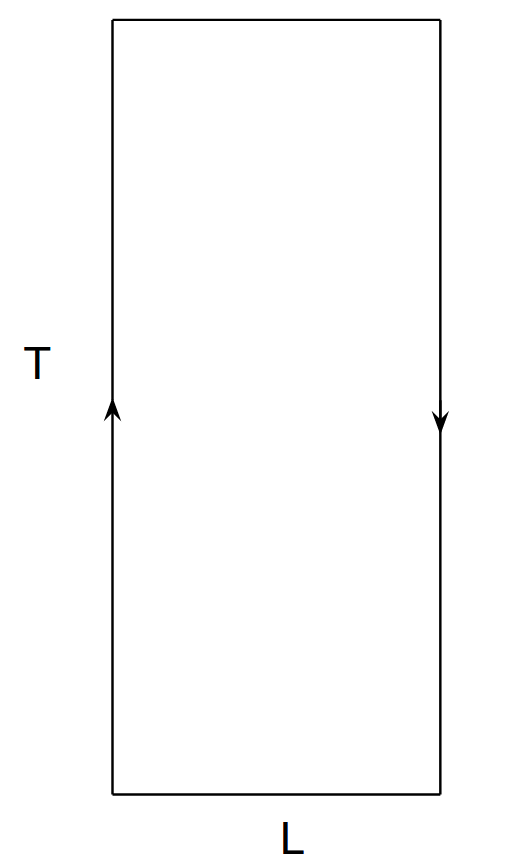
\includegraphics[width=4cm]{Images/WLrectangle.png}}
\end{center}
\caption{\label{fig:WLrectangle} Trajectory of a probe quark and antiquark separated by distance $L$, and travel $T$ distance in time. }
\end{figure}


We are interested in a supersymmetric extension of the Wilson loop,
such that it is computable through localization, see conditions \eqref{loc:susyCondition}.
We will study the so-called Maldacena-Wilson loop \cite{Maldacena:1998im},
where we add a coupling to the scalars of the vector multiplet:
\begin{equation} \label{maldacenaWL}
 U = \mathop{\mathrm{P}}\exp 
    \left[ 
	\int_C ds\,
	\left(
	  i\dot{x}^\mu A_\mu +|\dot{x}|n^I\Phi_I 
	\right)
    \right], \quad I=0,9.
\end{equation}
% where $n^I$ are components of the unit vector that parametrizes $S^5$.
Let us start by reviewing some known results in $\mathcal{N}=4$ SYM and then generalize them to $\mathcal{N}=2^*$.



\section{Wilson loops in $\mathcal{N}=4$ SYM}

The simplest Wilson loop is an infinite straight line. 
It is a half-BPS object, meaning it commutes with half of the 32 supercharges of $\mathcal{N}=4$ SYM.
This fact protects the Wilson line from quantum corrections and its value is simply one:
\begin{equation}
 \braket{W_\text{line}} = 1.
\end{equation}


By conformal transformation, the Wilson line can be mapped to a circular Wilson loop.
The result, however, is not the same. 
This is often referred to as a conformal anomaly, 
and it is due to the fact that large conformal transformations such as inversion are not symmetries in the flat space
(infinity is not a point of $\mathbb{R}^d$). 
On the sphere, these are symmetries, hence there is no distinction between a circle and a line, and the
expectation value of either is the same as for a circle on $\mathbb{R}^4$ \cite{Drukker:2000rr}.
The circular Wilson loop, which is also half-BPS, is exactly computable using the localized partition function for the theory on $S^4$,
where the path is the equator of sphere, see figure \ref{fig:equatorWL}.

\begin{figure}[t]
\begin{center}
 \centerline{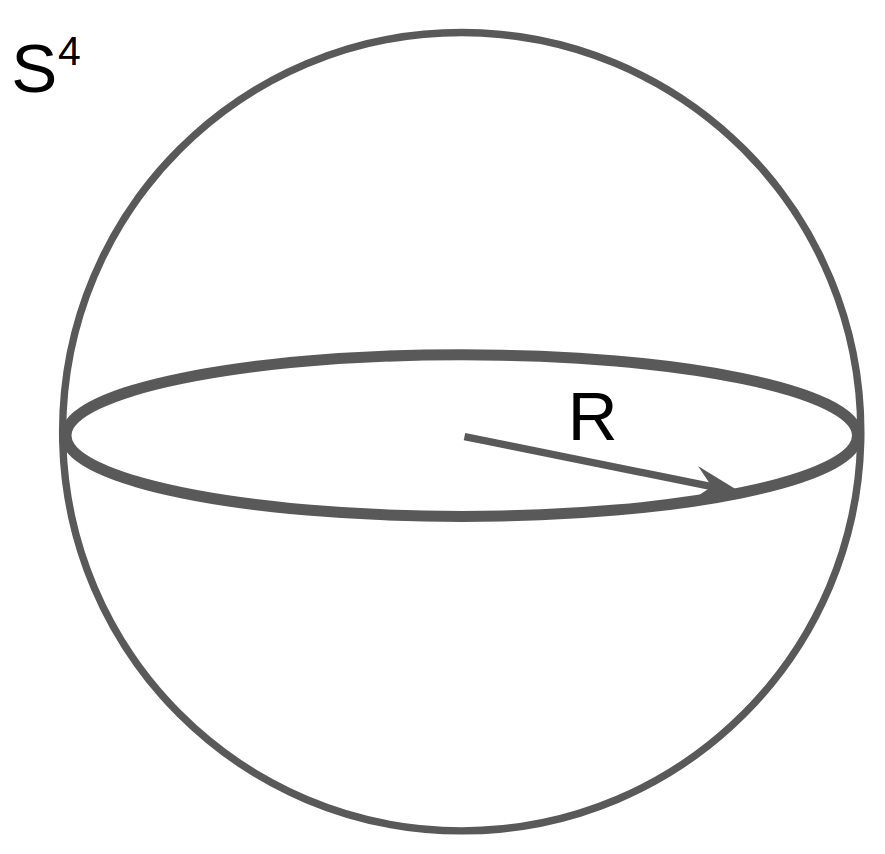
\includegraphics[width=4cm]{Images/equatorWL.png}}
\end{center}
\caption{\label{fig:equatorWL} The contour of the circular Wilson loop we study is the equator of the hypersphere the theory is defined on.}
\end{figure}


\subsection{Fundamental representation}
The circular Wilson loop in the fundamental representation is mapped to a matrix model expectation value:
\begin{equation}\label{eq:W1mm}
 W_1 = \left< \dfrac{1}{N}\sum_{i=1}^N e^{2\pi a_i} \right>_\text{matrix model},
%  \overset{N \gg 1}{\approx} \int_{-\mu}^{\mu} dx\, \rho(x) \,e^{2\pi x}
\end{equation}
which can be solved exactly for GUE \cite{Drukker:2000rr}:
\begin{equation}
 W_1 = \dfrac{1}{N} L_{N-1}^1 (-\lambda/(4N)) e^\frac{\lambda}{8N},
\end{equation}
where $L$ is the generalized Laguerre polynomial:
\begin{equation}
 L_n^m(x)=\dfrac{x^{-m}  e^x}{n!}\,  \dfrac{d^n}{dx^n}(e^{-x} x^{n+m}).
\end{equation}

In the large $N$ limit and fixed 't Hooft coupling, 
\eqref{eq:W1mm} can be written as:
\begin{eqnarray}
 W_1 &=& \int_{-\mu}^{\mu} dx\, \rho(x) \,e^{2\pi x} \label{eq:W1continuous} \\
     &=& \dfrac{2}{\sqrt{\lambda}} I_1 (\sqrt{\lambda}), \quad (N\rightarrow \infty \quad \text{and} \quad \lambda \text{ - fixed})
\end{eqnarray}
where for the last equality, we used the semicircle distribution \eqref{semicircle},
since the Wilson loop insertion to the partition function is subleading in $N$.
$I_1(x)$ is the modified Bessel function:
\begin{equation}
 I_1(x) = \sum_{n=0}^\infty  \dfrac{1}{n! (n+1)!} \left(\dfrac{x}{2}\right)^{2n+1}.
\end{equation}


Historically, the large-$N$ result was initially obtained by Erickson-Semenoff-Zarembo \cite{Erickson:2000af},
by summing over rainbow diagrams in perturbation theory, and they conjectured the Gaussian matrix model structure for $\mathcal{N}=4$ SYM.
Eventually Pestun's work in localization \cite{Pestun:2007rz} proved it.



In the 't Hooft limit, which is the holographic regime, 
\begin{equation}\label{W1holographic}
 W_1 = \sqrt{\frac{2}{\pi}} \lambda^{-3/4} e^{\sqrt{\lambda}}, 
 \quad (N\rightarrow \infty \quad \text{and} \quad \lambda \rightarrow \infty).
\end{equation}
% which matches with the minimal surface of the worldsheet with boundary $C$, drawn by the classical string on the supergravity background.
% We will discuss more on the holographic dual in another chapter.
% The subleading order term comes from the measure of the path integral, and so far, 
% it is still an open problem that many attempted to solve (cite Papers). 

% The equatorial Wilson loops can be generalized to latitude Wilson loops, 
% though the latter are less supersymmetric, and belongs to the family of 1/4 BPS.
% Their exact result can be obtained by just rescaling the 1/2 BPS, by 
% $\lambda \rightarrow \lambda \cos^2\theta_0$, 
% where the angle $\theta_0$ is the polar angle of the latitude.


\subsection{Higher rank representations}

Exact results for arbitrary representation of $U(N)$ can also be obtained \cite{Fiol:2013hna}.
These are very generic, though, 
but the generating function of $k$-antisymmetric representation 
\begin{equation}\label{eq:generatingFunctionAk}
 \braket{G_{A_k}(t)}=\sum_{k=0}^{N} t^k \, W_{A_k}
\end{equation}
has a nice compact form:
\begin{equation}
 \braket{G_{A_k}(t)}=\text{det}\left(t \delta_{ij}+ L_{i-1}^{j-i}(-\lambda/(4N)) e^{\frac{\lambda}{8N}}\right).
\end{equation}

We study the 't Hooft limit
for the symmetric (+) and the antisymmetric (-) representations. 
The generating functions\footnote{
Here, unlike in \eqref{eq:generatingFunctionAk}, 
we use the expansion parameter $e^{-\nu}$ instead of $t$.}
for the character of these representations are explicitly known:
\begin{equation}
 G_k^{\pm}(\nu) = \prod_{i=1}^N (1\mp e^{a_i - \nu})^{\mp}.
\end{equation}
Notice that these are also the Bose (+) and Fermi (-) distributions, in terms of the eigenvalues $a_i$.

The standard procedure is to derive the character by inverting the generating function using Cauchy's integral formula:
\begin{equation}\label{eq:characterIntegral}
 \chi_k^\pm \equiv \text{tr}_\pm \,U = \int_{C-i\pi}^{C+i\pi} \dfrac{d\nu}{2\pi i} \, e^{\nu k} G_k^\pm(\nu),
\end{equation}
where $C>a_i, \forall i$, for the symmetric case, and $C$ is arbitrary for the antisymmetric case.


All we need to do now is to compute the expectation value of the above integral. 
We can still employ the semicircle distribution \eqref{semicircle}, 
and we further take the large representation limit $k \sim N$,
which allows us to use the saddle-point method in \eqref{eq:characterIntegral}, \cite{Hartnoll:2006is}.
The saddle-point equation to solve for $\nu_*$ is
\begin{equation}\label{eq:saddlePointDensity}
 \dfrac{k}{N} = \int_{-\mu}^\mu dx \, \dfrac{\rho(x)}{e^{L(\nu_*-x)}\mp 1}, 
 \quad (N\rightarrow \infty \quad \text{and} \quad \frac{k}{N} \text{ - fixed}),
\end{equation}
which is analogous to the particle density equation in a Bose/Fermi system.

The final leading solutions for the antisymmetric representation is
\begin{equation}\label{solW-}
 \log W_{k}^-= N \frac{2\sqrt{\lambda }}{3\pi}\,\sin^3\theta, 
\end{equation}
where $\cos \theta\equiv \nu_*/\mu$ satisfies the transcendental equation
\begin{equation}\label{eqThetaAntisym}
 \theta -\frac{1}{2}\,\sin 2\theta =\pi \frac{k}{N},
\end{equation}
resulting from \eqref{eq:saddlePointDensity}
after the step-function approximation of the Fermi distribution.

For the symmetric representation, however, 
there is no saddle-point solution for \eqref{eq:saddlePointDensity}. 
This is the same phenomenon as the Bose-Einstein condensation.
It is possible to analytically continue the solution to the second Riemann sheet, though, 
as done in \cite{Hartnoll:2006is},
and the final result is:
\begin{equation}\label{solW+}
 \log W_{k}^+ = 2 N  f\left(\kappa\right),  
 \quad  \kappa \equiv \frac{\sqrt{\lambda }\,k}{4 \,N}
\end{equation}
where 
\begin{equation}\label{eqfSym}
 f(x) = x\sqrt{1+x^2}+\mathop{\mathrm{arcsinh}}x.
\end{equation}

The drawback of the analytic continuation was that computing large-$N$ corrections became less clear, as attempted in \cite{Faraggi:2014tna}.
In Paper II and Paper IV, we used a more systematic approach.
Paper IV focused exclusively on the symmetric Wilson loop in $\mathcal{N}=4$ SYM, 
where subleading corrections in $N$ were computed.
This result is consistent with the expansion of the known exact result for the multiply wrapped fundamental Wilson loop \cite{Kawamoto:2008gp},
which helped to clarify the apparent mismatch observed in \cite{Faraggi:2014tna},
and agrees with the analysis by \cite{Yamaguchi:2007ps} that symmetric representations and the multiply-wound fundamental ones 
differ by exponentially-suppressed terms in strong coupling.
Paper IV also derived the strong-coupling corrections, 
in response to the strong-coupling expansion done for the antisymmetric case in \cite{Horikoshi:2016hds},
where the Sommerfeld expansion of the Fermi distribution was used.
%k-fundamental obtained by relplacing $\lambda \rightarrow k^2 \lambda$.




\section{Wilson loops in $\mathcal{N}=2^*$ SYM}

The story can be extended to $\mathcal{N}=2^*$ SYM on $S^4$.
Here we have an extra parameter: the scale $MR$.
We will take the decompactification limit $MR \rightarrow \infty$, where interesting phase transitions were seen, 
and also, the dual theory is fully known on $\mathbb{R}^4$ \cite{Pilch:2000ue}.
% (the dual on $S^4$ is partially known, \cite{Bobev:2013cja}).

% We work with the equatorial circular Wilson loop and reasonably assume that results in the decompactification limit is universal for any large contour.


\subsection{Fundamental representation}

Since the fundamental Wilson loop is basically an exponentially-weighted integral \eqref{eq:W1continuous},
its value in the strong coupling limit is determined by the largest eigenvalue $\mu$
(recall $\mu\sim\sqrt{\lambda}$, see \eqref{semicircleN=2*}). 
Thus, we do not expect its strong coupling corrections to probe the cusps region.
In Paper I, we computed the subleading correction to the endpoint $\mu$,
which lead to the same correction to the Wilson loop (in terms of the perimeter $l=2\pi R$):
\begin{equation}\label{WLFundN2}
 \log W_1= P(\lambda) Ml, \quad P(\lambda) = \frac{\sqrt{\lambda}}{2 \pi} -\frac{1}{2} + \mathcal{O}\left(\dfrac{1}{\sqrt{\lambda}}\right), 
 \quad (MR\rightarrow \infty).
\end{equation}
The leading order term is the same as its homologous case in $\mathcal{N}=4$, only rescaled by $MR$ \cite{Buchel:2013id},
as a direct consequence of the semicircle behavior of the bulk distribution \eqref{semicircleN=2*}.
As a consistent check, when $M\rightarrow 0$, the Wilson loop goes to 1, as expected for the $\mathcal{N}=4$ case.
Moreover, we clearly see the perimeter law here since the theory is not confining neither conformal.



\subsection{Symmetric and antisymmetric representations}
In Paper II, result for symmetric and antisymmetric representations were computed,
up to the next-to-leading order in the strong coupling expansion.
The decompactified results at the leading order in $N$ are also the same as the ones in the $\mathcal{N}=4$ case,
but rescaled differently:
\begin{eqnarray}
 \log W_{k}^- &=& N M R\frac{2\sqrt{\lambda }}{3\pi}\,\sin^3\theta,\\
 \log W_{k}^+ &=& 2 N (MR)^2 f\left(\frac{\kappa}{M R}\right),
\end{eqnarray}
where $\theta$ and  $f$ satisfy the same equation as in \eqref{eqThetaAntisym} and \eqref{eqfSym}, respectively.

Now, the interesting part lays in the subleading terms. 
Unlike the fundamental representation, the higher rank representations do probe the endpoint distribution of the eigenvalues, 
which has periodic cusps with period $MR$, see figure \ref{fig:phaseDiagram}.
The results are:
\begin{equation}\label{WantisymPW}
 \delta \log W_{k}^- = -\dfrac{2\pi^2}{3} \dfrac{N M R}{\lambda^{3/4}}
\begin{cases}
 4\tilde{f}^3 & {\rm }0<\tilde{f}\leq 1
\\
 \tilde{f}^3+6\tilde{f}-\frac{3}{\tilde{f}} & {\rm } 1<\tilde{f}\leq 1+\sqrt{2}
 \\
 \vdots &
\end{cases}, \quad 
\tilde{f} = \dfrac{\lambda^{3/4} k }{ 4\sqrt{\pi} N}
\end{equation}
and
\begin{equation}\label{WsymPW}
 \delta \log W_{k}^+ = \dfrac{2^5\pi^{3/2}}{5}\dfrac{N (M R)^2}{\lambda^{3/4}} \left(v^{5/2}+\Theta(v-1)\left(v+\dfrac{2}{3}\right)(v-1)^{3/2}\right), 
\end{equation}
where $\Theta(x)$ is the Heaviside function and $v$ is written in terms of the scaling parameter $\tilde{f}$ as
\begin{equation}
  \dfrac{3}{2}\tilde{f} = v^{3/2}-\Theta(v-1)(v-1)^{3/2}, \quad \tilde{f} = \dfrac{\lambda^{3/4} k}{8\sqrt{\pi} M R N}.
\end{equation}
The solutions are plotted in figure \ref{fig:plotsCorrection}.
The phase transitions are of second and third order for the antisymmetric and symmetric representations, respectively,
in the sense that the derivatives of the free energy $F=-\frac{1}{N}\log W$ with respect to $\tilde{f}$ exhibit discontinuity at these orders.

% \begin{figure}[t]
% \begin{center}
%   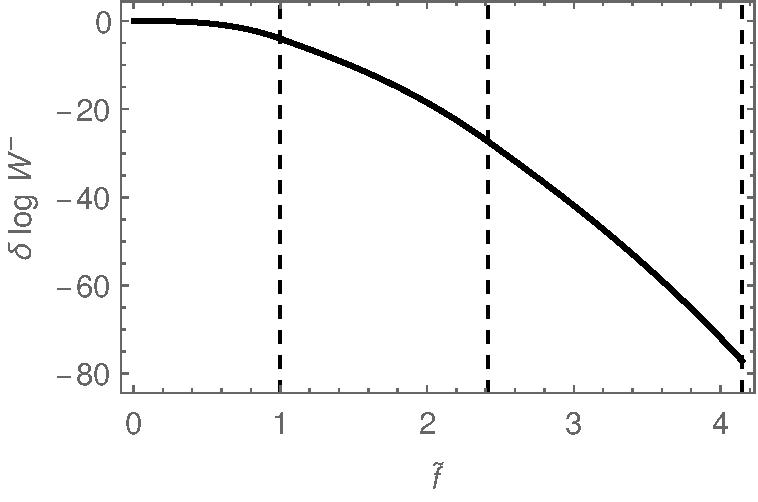
\includegraphics[width=0.49\textwidth]{Images/AntisymBlack.pdf} 
%   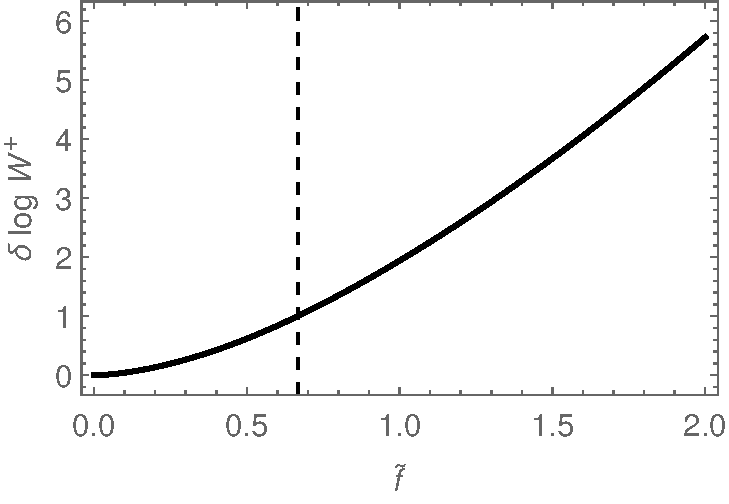
\includegraphics[width=0.49\textwidth]{Images/SymBlack.pdf} 
% \end{center}
% \caption{\label{fig:plotsCorrection} Strong coupling correction for the (rescaled) log of Wilson loops in 
% antisymmetric representation (left) with the critical points at $\{1, 1+\sqrt{2}, 1+\sqrt{2}+\sqrt{3},\ldots\}$,
% and in symmetric representation (right) with the critical point at $2/3$.}
% \end{figure}

\begin{figure}[t]
\begin{center}
 \centerline{ 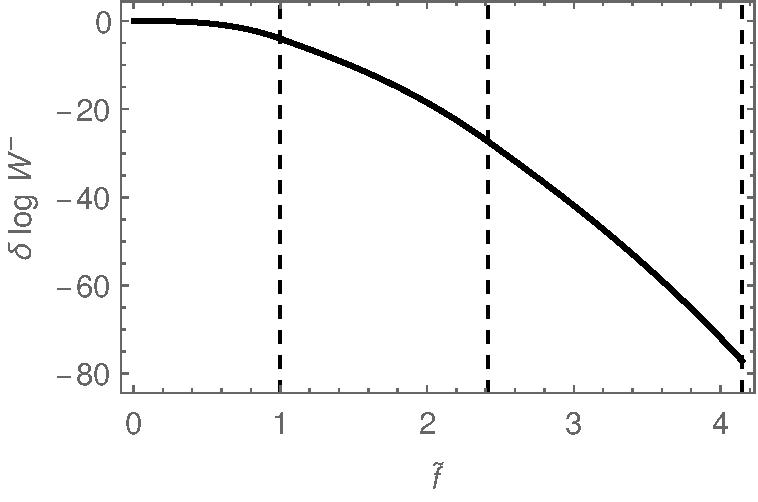
\includegraphics[width=0.8\textwidth]{Images/AntisymBlack.pdf} }
 \centerline{ 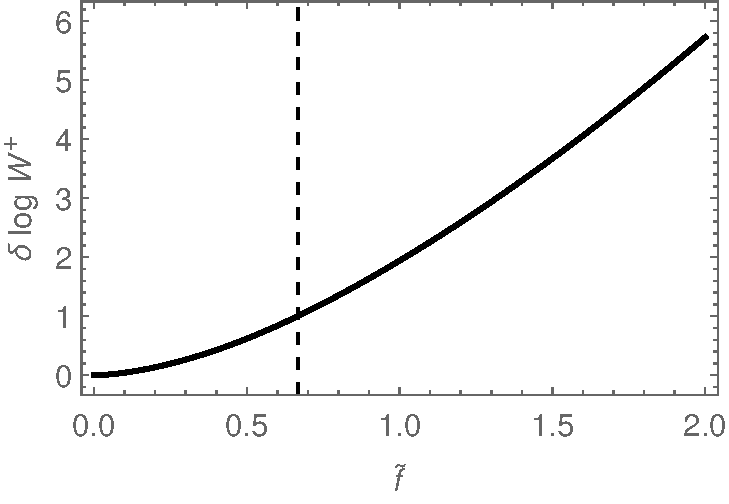
\includegraphics[width=0.8\textwidth]{Images/SymBlack.pdf} }
\end{center}
\caption{\label{fig:plotsCorrection} Strong coupling correction for (rescaled) log of Wilson loops in 
antisymmetric representation (up) with the critical points at $\{1, 1+\sqrt{2}, 1+\sqrt{2}+\sqrt{3},\ldots\}$,
and in symmetric representation (down) with the critical point at $2/3$.}
\end{figure}


   \part{Gauge/string duality}
     \chapter{Supergravity }\label{ch:supergravity}


Quantum gravity theories must contain massless spin 2 particles, that are gravitons.
In the same fashion as we built super-Yang-Mills (SYM) theories, with maximum spin 1,
we can build supergravity (SUGRA) theories by requiring the supermultiplet to contain gravitons (and no higher spin particles).
This constrains the number of super-Poincar\'e charges to a maximum of 32\footnote{
In the unitary massless spinor representation $S$, half of the supercharges annihilates the highest weight state.
Only half of the remaining supercharges are spin-raising operators (the other half lowers spin).
On the hand, we can have at most 8 raising operators from spin -2 to 2 by steps of 1/2. 
Then (see e.g. \cite{DHoker:2002nbb}), for $\mathcal{N}$ copies of supersymmetries:
\[
1/4 \times \mathcal{N} \times \text{dim } S = 8 
\quad \Rightarrow \quad
\mathcal{N}  \text{dim } S = 32.
\]
}.


For one copy of supersymmetry, i.e. $\mathcal{N} = 1$, 
we have a unique supergravity theory in 11 dimensions \cite{Cremmer:1978km}, 
from which many lower dimensional supergravity theories can be obtained by the means of 
Kaluza-Klein compactication and dimensional reduction.
This theory contains a metric, an antisymmetric rank 3 tensor and a Majorana gravitino field.


Compactifying it on a circle and taking its radius to be zero, 
we obtain type IIA $\mathcal{N}=2$ SUGRA in 10 dimensions,
which is also a low energy effective action of type IIA superstring theory.
Using T-duality\footnote{
It states that strings compactified on a torus with radius $R$ is equivalent to strings compactified on a torus with
radius proportional to $1/R$.}, 
we can obtain type IIB $\mathcal{N}=2$ SUGRA,
% which is chiral (i.e. violates parity).
which is of our interest to study the AdS/CFT duality.
Let us list its field content:
\begin{center}
 \begin{tabular}{ |l | l| }
  \hline
  rank 2 symmetric tensor: metric & $g$ \\  \hline
  complex scalar: axion-dilaton  & $C_{(0)} + i \,e^{-\Phi}$ \\ \hline
  rank 2 antisymmetric tensor & $C_{(2)} + i \, B_{(2)}$ \\ \hline
  rank 4 antisymmetric tensor & $C_{(4)}$\\\hline
  Majorana-Weyl $3/2$-spinor: gravitinos & $\psi_M^I, \: I=1,2 $\\\hline
  Majorana-Weyl $1/2$-spinor: dilatinos & $\lambda^I, \: I=1,2 $ \\\hline
\end{tabular}
\end{center}
The gauge potentials $C_{(i)}$ are called the Ramond-Ramond potentials.
% The theory does not have a manifestly Lorentz-invariant action principle, it does have covariant field equations.
The fields above must satisfy the supergravity equations that consist of \cite{Schwarz:1983qr}:
\begin{itemize}
 \item Einstein's equations
 \item Maxwell's equations
 \item The dilaton equation
 \item (Hodge) self-duality equation: $*F_{(5)} = F_{(5)}$,  where \\
	\begin{equation} \label{5form}
	 F_{(5)} = dC_{(4)} - \dfrac{1}{2} C_{(2)}\wedge dB_{(2)} + \dfrac{1}{2} B_{(2)} \wedge dC_{(2)}.
	\end{equation}
\end{itemize}
To avoid introducing more notation, we refer the reader to e.g. \cite{Buchel:2000cn} 
for explicit expressions of the above equations.

The supersymmetry condition imposes the variation of dilatinos and of gravitinos to be zero \cite{Schwarz:1983qr}.
These are Killing equations and by solving them we obtain the Killing spinors of the background geometry.
For $AdS_5 \times S^5$, the solutions can be found in \cite{Skenderis:2002vf},
and for the Pilch-Warner background, see \cite{Pilch:2003jg} and the appendix D of Paper III.


\section{$AdS_5 \times S^5$}
The simplest solution to the supergravity equations is $AdS_5 \times S^5$ geometry,
where the dilaton $\Phi$, the $B$-field and the gauge potentials $C_{(0)}$ and $C_{(2)}$ are trivial.
% and it has the (Ramond-Ramond) 5-form flux \eqref{5form}.

Since spheres are more familiar, let us review only the metric of the anti-de-Sitter space ($AdS$).
It is a hyperboloid with Minkowski signature, embedded in the flat space of one dimension higher, i.e.:
% The Anti-de-Sitter spacetime of $D+1$-dimension ($AdS_{D+1}$) is a maximally symmetric solution of vacuum Einstein's equation with negative cosmological constant.
% In D+2 dimensions with signature $(-,-,+,\ldots,+)$, it is naturally embedded in the flat space 
\begin{equation}
 ds^2 = -dX_0^2-dX_D^2+\sum_{i=1}^{d-1} X_i^2
\end{equation}
with the constraint 
\begin{equation} \label{hyperboloid}
 - X_0^2 - X_d^2 + \sum_{i=1}^{d-1} X_i^2 = - L^2.
\end{equation}
Figure \ref{fig:AdS} shows an example for $AdS_2$.
The isometry group is clearly $SO(2,d)$.

By solving the constraint, the induced metric (in global coordinates) for $AdS_{d+1}$ becomes:
\begin{equation}
 ds^2 = L^2(-\cosh^2 \rho d\tau^2 + d\rho^2+\sinh^2\rho d\Omega_{d-1}^2).
\end{equation}
where $d\Omega_{d}^2$ is the metric of $S^d$, $\rho\geq 0$ and $2\pi \geq \tau \geq 0$.

Another set of solutions that solve the constraint \eqref{hyperboloid} is the Poincar\'e coordinates.
These are preferred for holographic studies, 
since the metric in these coordinates 
\begin{equation}\label{metricAdS}
 ds^2 = \dfrac{L^2}{z^2} (\eta_{\mu\nu} dx^\mu dx^\nu+dz^2 ) 
\end{equation}
is manifestly conformal invariant, with flat space slicing for any $z>0$ (see figure \ref{fig:AdS}), 
despite it covers only half of the geometry.
% The metric for $AdS_5\times S^5$ in the Poincar\'e patch is:
% \begin{equation}\label{metricAdS5S5}
%  ds^2_{AdS_5\times S^5} = \dfrac{L^2}{z^2} (-dt^2+d\mathbf{x}^2+dz^2 ) + L^2 d\Omega_5.
% \end{equation}
The conformal boundary\footnote{
The boundary of $AdS$ is infinitely far aways from the bulk,
but it can be mapped to a finite distance using a conformal transformation.} 
corresponds to $z \rightarrow 0$, 
and $z$, called radial coordinate, is interpreted as the energy scale of the boundary theory in AdS/CFT.
% This statement is made more clear using holographic renormalization, see e.g. the lectures \cite{Skenderis:2002wp}.

\begin{figure}[t]
\begin{center}
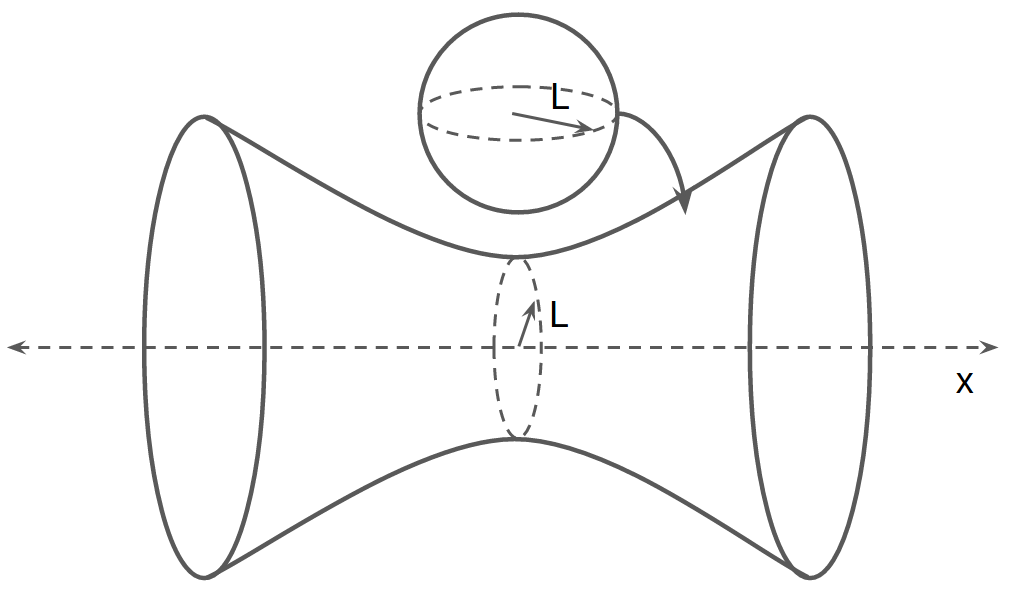
\includegraphics[width=0.49\textwidth]{Images/AdS2xS2.png}
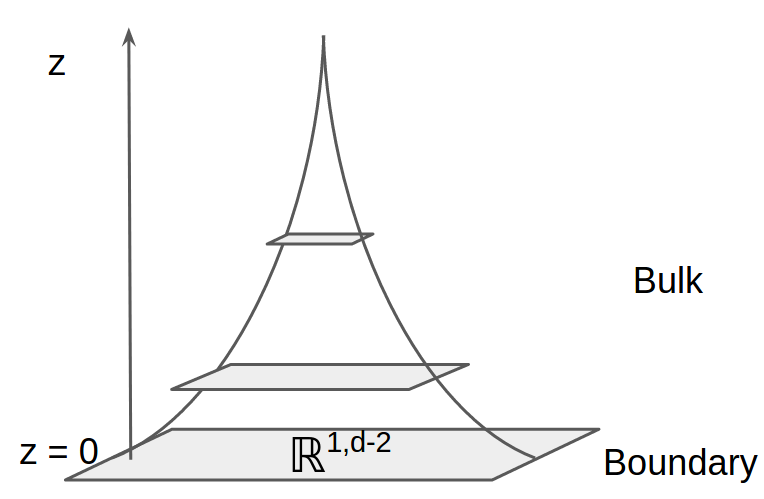
\includegraphics[width=0.49\textwidth]{Images/AdSPoincare.png}
\end{center}
\caption{\label{fig:AdS} Left: $AdS_2\times S^2$, where $AdS_2$ is defined by $x^2-y^2-t^2 = - L^2$, 
and at all its surface points we find the sphere.
Right: Flat space slicing for $AdS_d$ in Poincar\'e coordinates.}
\end{figure}

\section{D-branes}

D-branes are soliton-like solutions of the supergravity equations 
that preserve half of the 32 background supercharges (BPS solutions), see textbook \cite{Ammon:2015wua}:
\begin{eqnarray}
 ds^2   &=& H_p(r)^{-1/2} \eta_{\mu\nu}dx^\mu dx^\nu +  H_p(r)^{1/2} \delta_{ij} dy^i dy^j\\
 e^\Phi &=& g_s H_p(r)^{(3-p)/4}\\
 C_{(p+1)}&=&(H_p(r)^{-1} - 1) dx^0\wedge\cdots\wedge dx^p\\
 B_{(2)} &=& 0,
\end{eqnarray}
where $x^\mu, \mu=1,\ldots, p$ are the D-brane worldvolume coordinates, 
$y^i, i=p+1,\ldots,9$ are the transversal directions to the brane,
and the harmonic function is
\begin{equation}
 H_p(r) = 1 + \left( \dfrac{L_p}{r}\right)^{7-p}.
\end{equation}

It is intuitive to think of these solutions as charged point-like particles from the $(9-p)$-dimensional transverse space point of view.
For $N$ coincident D-branes, their total charge is proportional to $N$,
and from the Gauss law, we obtain
\begin{equation}
 N \propto \int_{S^{9-p-1}} *F_{(p+2)},
\end{equation}
quantizing therefore the (Hodge dual) of the flux of the Ramond-Ramond field $C_{(p+1)}$ through the hypersphere, $F_{(p+2)}$.
The above relation also determines the characteristic length scale 
\begin{equation}\label{characteristicLengthLp}
 L_p^{7-p} = (4\pi)^{(5-p)/2} \Gamma \left(\dfrac{7-p}{2}\right) g_s N \alpha'^{(1-p)/2},
\end{equation}
where $g_s$ is the string length and $\alpha'$ is the Regge slope. 
We will comment on these parameters in chapter \ref{chp:AdSCFT},
where we will also see that $AdS_5 \times S^5$ geometry can be obtained as the near horizon geometry of a stack of $N$ coincident D3-branes.

To conclude this section, 
let us write down the generic action of a single D-brane in Minkowski signature, 
which will be used later on in the thesis.
The action consists of the Dirac-Born-Infeld (DBI) term:
\begin{equation}\label{DBI}
 S_\text{DBI} = -T_\text{Dp} \int_M\,  d^{p+1}\xi e^{-\Phi} \, \sqrt{-\text{det}\left( P[g] + P[B] + \dfrac{1}{T_\text{F1}} F \right)},
%  d^{p+1}\sigma \,
\end{equation}
and the Wess-Zumino (WZ) term with the Ramond-Ramond potentials pulled back to the worldvolume:
\begin{equation}\label{WZ}
 S_\text{WZ} = T_\text{Dp} \int_M\, \exp{\left(B + \dfrac{1}{T_\text{F1}} F \right)} \wedge  P[C].
\end{equation}
The couplings are
\begin{equation} \label{couplingsTension}
 T_\text{F1} = \dfrac{1}{2\pi\alpha'},
 \quad 
 T_\text{D1} = \dfrac{1}{g_s}\,T_\text{F1},
 \quad 
 T_\text{Dp} =  T_\text{D1}\left(2\pi \sqrt{\alpha'}\right)^{1-p}.
\end{equation}
% and we use the replacement rules $\alpha'\rightarrow 1/\sqrt{\lambda}$ and $g_s \rightarrow \lambda/(4\pi N)$ 


\section{Pilch-Warner geometry}
Another solution that preserves $\mathcal{N}=2$ supersymmetric flow is found by Pilch-Warner \cite{Pilch:2000ue}.
The geometry is a deformed and warped $AdS_5 \times S^5$, and all the fields are non-trivial in this case.
The metric (in Einstein frame) is
% \footnote{
% The string metric $g$ and the Einstein metric $G$ are related by $g=e^{-\frac{4 \Phi }{D-2}} G$,
% where $\Phi$ is the dilaton.
% }
\begin{eqnarray}\label{metricPW}
 ds^2 & = & \dfrac{(c \, X_1 X_2)^{1/4}}{\sqrt{A}} L^2
	\left( 
	  \dfrac{M^2 A}{c^2-1} \eta_{\mu\nu}dx^\mu dx^\nu + \dfrac{1}{A (c^2-1)^2} dc^2 
	\right.\\
      & & +\left. \left[
		  \dfrac{1}{c} d\theta^2 + \dfrac{\sin^2\theta}{X_2} d\phi^2 
		  + \cos^2\theta  \left(\dfrac{A}{X_1}(\sigma_1^2 +\sigma_2^2) + \dfrac{A}{c \, X_2} \sigma_3 \right)  
		\right] 
        \right),\nonumber
\end{eqnarray}
where $\sigma_i, i=1,2,3$ are the Maurer-Cartan forms for $SU(2)$ and
\begin{eqnarray*}
 & X_1(c,\theta) =  \cos^2\theta + c\, A(c)  \sin^2\theta, \\
 &  X_2 (c,\theta)=  c \cos^2\theta + A(c)  \sin^2\theta, \\
 & A(c)  = c+\dfrac{1}{2}(c^2 - 1)\log\left(\dfrac{c-1}{c+1}\right).
\end{eqnarray*}
It reduces to $AdS_5 \times S^5$ near the boundary, i.e. expand the metric for $c \approx 1 + z^2 M^2/ 2$, 
where $z$ is the radial coordinate in \eqref{metricAdS}, then set $M=0$.

The Pilch-Warner solution is dual to $\mathcal{N}=2^*$ SYM on $\mathbb{R}^4$. 
% It is obtained using holographic renormalization for a truncated $\mathcal{N} = 8$ 5-dimensional SUGRA.
% That is, imposing supersymmetric  an asymptotic $AdS_5$ metric ansatz  and then lifted to 10d supergravity. 
Similarly the dual for $\mathcal{N}=2^*$ on $S^4$ has been studied in \cite{Bobev:2013cja},
but the solution is partially known only.
We are interested in the flat space regime, where interesting physics happen such as the phase-transitions discussed in Part I (see figure \ref{fig:phaseDiagram}).
Hence, the dual computations will be done in the Pilch-Warner background.





% \section{AdS geometry}
% 
% The Anti-de-Sitter spacetime of $D+1$-dimension ($AdS_{D+1}$) is a maximally symmetric solution of vacuum Einstein's equation with negative cosmological constant.
% In D+2 dimensions with signature $(-,-,+,\ldots,+)$, it is naturally embedded in the flat space 
% \begin{equation}
%  ds^2 = -dX_0^2-dX_D^2+\sum_{i=1}^{D-1} X_i^2
% \end{equation}
% with the constraint 
% \begin{equation}
%  - X_0^2 - X_D^2 + \sum_{i=1}^{D-1} X_i^2 = - l^2.
% \end{equation}
% The isometry group is $SO(2,d)$
% If the D dimension were Euclidean, the previous equation is a two-sheeted hyperboloid.
% (figures)
% 
% The constraint is solved by
% \begin{equation}
%  X_0 = l \cosh \rho \cos \tau , \quad 
%  X_D = l \cosh \rho \sin \tau , \quad 
%  X_i=l \eta_i \sinh \rho
% \end{equation}
% where the angles $\eta_i$ are such that $\sum_{i=1}^{D-1} \eta_i = 1$, 
% and $\rho\geq 0$ and $2\pi \geq \tau \geq 0$.
% \begin{equation}
%  ds^2 = l^2(-\cosh^2 \rho d\tau^2 + d\rho^2+\sinh^2\rho d\Omega_{d-1}^2).
% \end{equation}
% These new parameters form the global coordinates of AdS, since they cover the full hyperboloid.
% 
% There is another set of solutions that cover only half of the hyperboloid:
% \begin{eqnarray}
%  X_0 &=& \dfrac{1}{2}(z+\dfrac{1}{z}(l^2+\mathbf{x}^2 - t^2))\\
%  X_D &=& \dfrac{1}{2}(z-\dfrac{1}{z}(l^2-\mathbf{x}^2 + t^2))\\
%  X_1 &=& \dfrac{l}{z} t\\
%  X_i &=& \dfrac{l}{z} r
% \end{eqnarray}
% We call the above solution the Poincar\'e patch, and the metric is
% \begin{equation}
%  ds^2 = \dfrac{l^2}{z^2} (-dt^2+d\mathbf{x}^2+dz^2 )
% \end{equation}
% This form is manifestly conformal invariant, and is very useful for holographic computations.
% The conformal boundary corresponds to $z \rightarrow 0$.
% 
% % spherical geometry?
% % 
% % Killing spinor?






  

     \chapter{AdS/CFT correspondence}\label{chp:AdSCFT}


We have seen that a Yang-Mills theory with gauge group $U(N)$ is characterized by two parameters: 
the Yang-Mills coupling $g_\text{YM}$ and the gauge group rank $N$.
Before stating the gauge/string duality, also known as the holographic principle, 
let us discuss different perturbative limits in string theory.

In string theory, there are two parameters used for expansion: 
the string coupling constant $g_s$ and the string length\footnote{
It is a fundamental scale in string theory, and not literally the length of the strings.} $l_s = \sqrt{\alpha'}$.
% where $\alpha'$ is called the Regge slope, 
% and it is related to the string tension $T_\text{F1}=1/(2\pi\alpha')$.
When the string coupling is small, it leads to classical strings,
where only tree level diagrams are taken into account.
This means strings do not merge and split, 
which would give different worldsheet topologies, see figure \ref{fig:stringPerturbation}.
If the strings propagate in a curved background with a characteristic length scale $L$,
the classical gravity limit is obtained by requiring additionally $l_s \ll L$.
In other words, strings can be approximated by point particles (their center mass). 

\begin{figure}[t]
\begin{center}
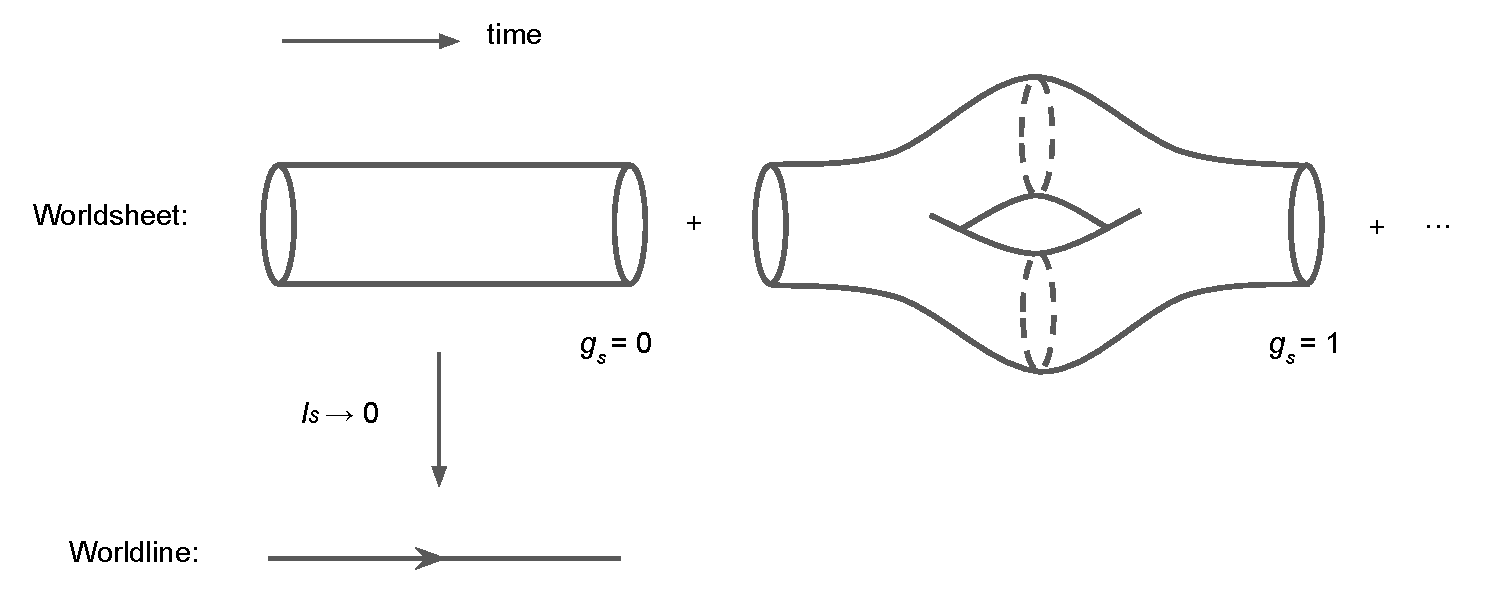
\includegraphics[width=\textwidth]{Images/stringPerturbation.pdf}
\end{center}
\caption{\label{fig:stringPerturbation} Genus expansion of the closed string worldsheet and the point-particle approximation.}
\end{figure}


The AdS/CFT correspondence was originally conjectured by Maldacena \cite{Maldacena:1997re}, 
and stated the below theories are dynamically equivalent:
\begin{itemize}
 \item $\mathcal{N}= 4$ SYM in 4 dimensions with gauge group $SU(N)$
 \item Type IIB superstring theory on $AdS_5 \times S^5$ (both with the same radius L), 
       where the $F_{(5)}$ has integer flux $N$ on $S^5$.
\end{itemize}
The parameters of these two theories are related as:
\begin{equation}\label{couplings}
 g_\text{YM}^2 = 4 \pi g_s, \quad  \lambda \equiv g_\text{YM}^2 N = \left(\dfrac{L}{l_s}\right)^4.
\end{equation}

The conjecture was further developed by \cite{Gubser:1998bc, Witten:1998qj},
and since its original inception, other examples have been found such as
a lower dimensional correspondence between a 3d CFT called ABJM theory 
and type IIA superstring on $AdS_4 \times CP^3$ \cite{Aharony:2008ug}, known as $AdS_4/CFT_3$ correspondence.
It is also an active field of research, but here, we will focus only on the $\mathcal{N}= 4$ case.



We see the first relation in \eqref{couplings} implies the YM's coupling to be small in the classical strings limit.
Moreover, from the second relation, $L/l_s $ is arbitrary in this limit, 
hence $N$ must be large to compensate the smallness of $g_\text{YM}$.
The 't Hooft coupling $\lambda $ is then kept fixed when $N$ is large.
This limit gives planar Feynman diagrams, see figure \ref{fig:planarNonPlanar}, in the leading order on the gauge theory side, 
and corresponds to the genus expansion in string worldsheet, see figure \ref{fig:stringPerturbation}.
This was actually noticed by 't Hooft long before the advent of AdS/CFT correspondence \cite{tHooft:1973alw},
and suggested planar diagrams as triangulations of the string worldsheet.
Notice that, in the planar limit, the Lie groups $U(N)$ and $SU(N)$ are indistinguishable.
% the same, and differ at higher orders in $1/N^2$. 
% It is actually not completely clear which one of these is the gauge group in the correspondence.

\begin{figure}[t]
\begin{center}
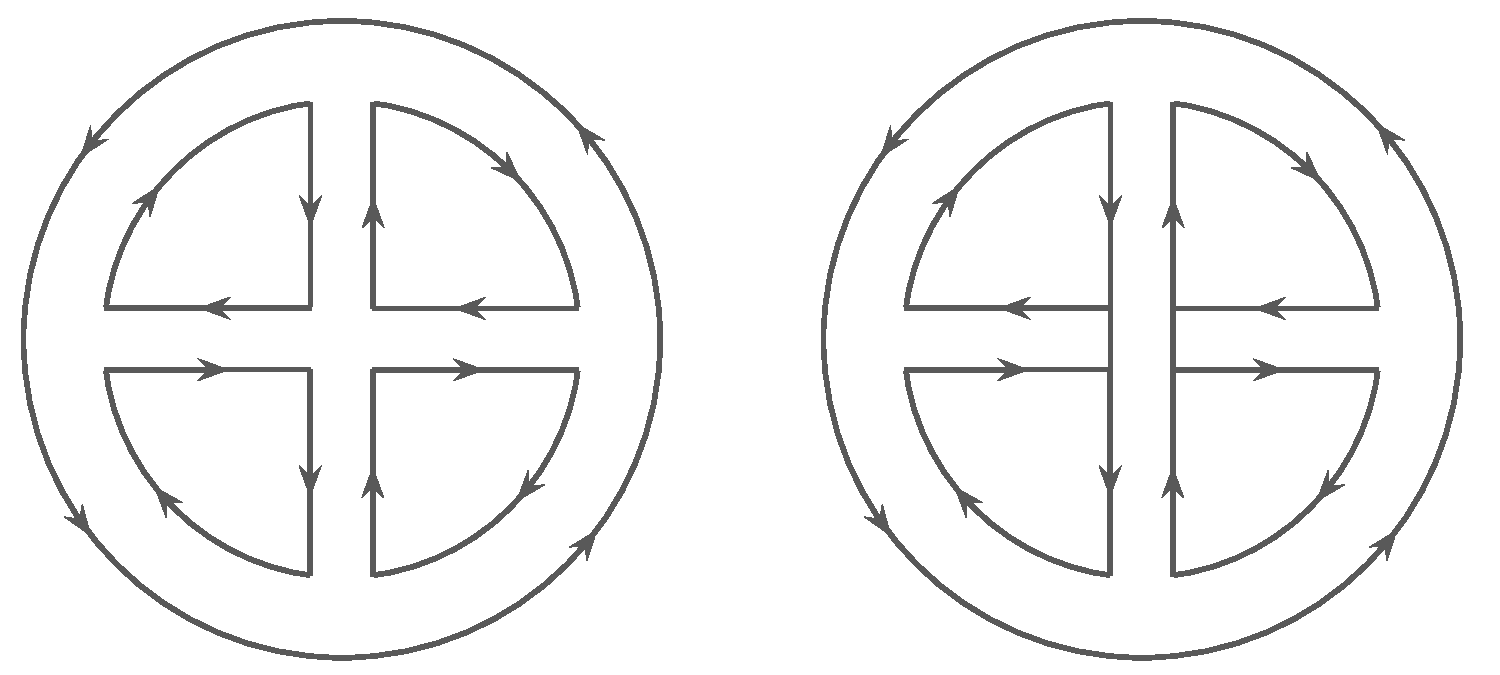
\includegraphics[width=0.7\textwidth]{Images/planarNonPlanar.pdf}
\end{center}
\caption{\label{fig:planarNonPlanar} A planar diagram (left) and a non-planar diagram (right).}
\end{figure}


If we further impose classical gravity limit, then
the 't Hooft coupling must be large too. 
Hence, the correspondence becomes a form of strong/weak duality.
This is the 't Hooft limit and it is the most computationally accessible one, 
since our understanding of string theory beyond the above-mentioned perturbative regimes is poor. 
Moreover, it is potentially seen as a tool to solve strongly coupled quantum field theory using supergravity.
Let us summarize the different limits in the table below:
\begin{center}
 \begin{tabular}{| l | l |}
 \hline
  $\mathcal{N}=4$ SYM & Type IIB strings on $AdS_5 \times S^5$ \\ \hline
  $N, \quad \lambda = g_{YM}^2 N$            & $g_s = \frac{\lambda}{4\pi N}, \quad T = \frac{\sqrt{\lambda}}{2 \pi} $ \\ %(quantum superstring) \\
  $N\rightarrow \infty, \quad \lambda$ fixed & $g_s=0, \quad T$ fixed \\  %(classical superstring) 
  $N\rightarrow \infty, \quad \lambda \rightarrow \infty$ & $g_s=0, \quad T \rightarrow \infty$ \\\hline %   (classical supergravity )
%    Local operators & String states  \\
\end{tabular}
\end{center}

Symmetry-wise, the conjecture is consistent:
\begin{center}
 \begin{tabular}{| l | l |}
 \hline
  $\mathcal{N}=4$ SYM    & Type IIB strings on $AdS_5 \times S^5$ \\ \hline
   conformal symmetry $SO(4,2)$   & isometry of $AdS_5$: $SO(4,2)$ \\ 
   R-symmetry $SO(6)$             & isometry of $S^5$: $SO(6)$ \\ 
   SUSY: 32 supercharges          & SUSY: 32 supercharges \\ \hline
%    Local operators & String states  \\
\end{tabular}
\end{center}

As for local operators in CFT, the AdS/CFT statement is that\footnote{It is generalized to asymptotic $AdS$ spaces, such as the Pilch-Warner geometry.}
\begin{equation}
 \int_{\phi\sim\phi_{(0)}} D\phi e^{-S_\text{string}[\phi]} = \braket{e^{-\int_{\partial AdS} \phi_{(0)} O }}_{CFT},
\end{equation}
where $\phi_{(0)}$ represents the boundary values of fields $\phi$ living in the bulk of $AdS$.
In the supergravity limit, the on-shell supergravity action corresponds to the generating function of connected graphs in the field theory.
In other words, bulk fields with non-trivial boundary values are sources of gauge invariant operators in CFT.
Since the volume of $AdS$ is infinite (due to the second order pole in the radial coordinate),
the divergences are removed using \emph{holographic renormalization}, 
which is analogous to the renormalization of correlation functions.
Holographic renormalization consists of expanding bulk fields close to the boundary, 
identifying the divergent terms and remove them by counterterms, as in the usual renormalization procedure, see e.g. \cite{Skenderis:2002wp} for a review.
% This is also the procedure used to find the holographic dual of N=2*, 
% by solving the non the asymptotic AdS spaces such as Pilch-Warner geometry. 

A formal proof of AdS/CFT correspondence is yet elusive, despite numerous explicit checks.
Next, we will review the original argument from \cite{Maldacena:1997re}.

% \section{Holographic re}


\section{N D3-branes}

The origin of this correspondence lies on the two perspectives of D-branes in superstring theory.

D-branes are non-perturbative objects where open strings end (with Dirichlet conditions, i.e. fixed endpoint with zero momentum). 
In the weak coupling limit $g_s \ll 1$, 
open strings can be thought as excitations of D-branes, see e.g. figure \ref{fig:2Dbranes}.
In the low energy limit $E \ll 1/l_s$, the massive string excitations can be ignored.

Consider a single D3-brane and let us expand its action (the DBI part) for $l_s \ll 1$, 
which gives the low energy open (bosonic) string action:
\begin{equation}
 S = - \dfrac{1}{2 \pi g_s} \int d^{4}x \, (1+\dfrac{1}{4} F^{\mu \nu} F_{\mu \nu} 
     + \dfrac{1}{2} \partial_\mu \Phi_I \partial^{\mu} \Phi^I +\ldots). %+ \mathcal{O}(\alpha'))
\end{equation}
These fields are the gauge field $F_{\mu \nu}$ that transforms in the unbroken Lorentz symmetry of the 4-dimensional worldvolume,
% indexed by $\mu, \nu = 1,2,3$,
and massless scalar fields $\Phi^I$  that are Goldstone bosons of the broken translation symmetry in the six transverse directions of the target space,
due to the presence of the brane. 
The resulting effective theory (excluding the term with no fields) is a $U(1)$ gauge theory living in the worldvolume of the D3-brane.
This identifies the string coupling constant with the Yang-Mills coupling: $4 \pi g_s = g_\text{YM}^2$.
The gauge group is $U(1)$ for a single D-brane, and for $N$ D-branes, 
it gets enhanced from $U(1)^N$ to $U(N)$ if they are coincident, see explanations in \cite{Wulff:2007vj}.
The effective coupling constant is then given by $g_s N$.
% Therefore, this perspective is only reliable for $g_s N \ll 1$.
The full spectrum also contains closed string modes and interaction terms, 
but by carefully taking the low energy limit, these sectors decouple and the interaction term vanishes.

\begin{figure}[t]
\begin{center}
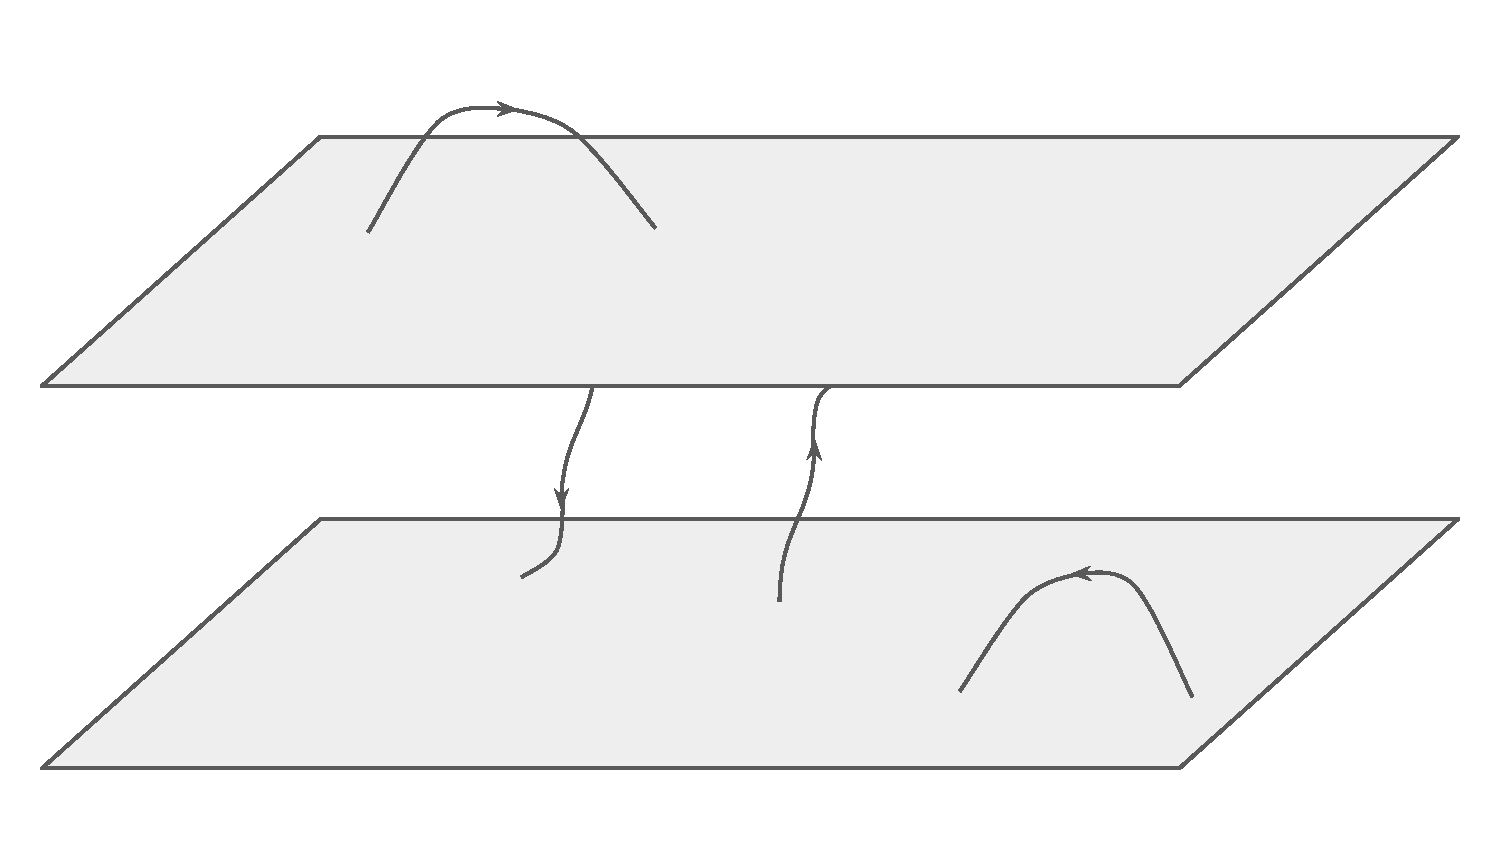
\includegraphics[width=0.6\textwidth]{Images/2Dbranes.pdf}
\end{center}
\caption{\label{fig:2Dbranes} All the possible (oriented) open string excitations in two D-branes. 
If we have $N$ non-coincident D-branes, then there are $N^2$ possible open string configurations.}
\end{figure}

% If we have N non-coincident D-branes, then there are $N^2$ possible open string configurations characterized by their endpoints
% (e.g. for $$\mathcal{N}=2$$, we have (1,1), (1,2), (2,1), (2,2), where the tuple represents the two branes).
% These can be encoded in a $N\times N$ matrix. 

On the other hand, D-branes are also solutions of supergravity field equations, as discussed in chapter \ref{ch:supergravity}.
Hence, as gravitational objects, they can deform the surrounding spacetime, and closed strings can propagate there.
% The supergravity limit is a low energy limit of superstring theory. 
For a stack of $N$ coincident D3-branes, the metric is
\begin{equation}
 ds^2 = \left( 1 + \dfrac{L^4}{r^4} \right)^{-1/2} \eta_{i j} dx^i dx^j  + \left( 1 + \dfrac{L^4}{r^4} \right)^{1/2} (dr^2 + r^2 d\Omega_5^2).
\end{equation}
Notice the two limits for this metric:
\begin{itemize}
 \item $r \gg L$: leading to the 10-dimensional flat Minkowski metric.
 \item $r \ll L$: redefining $z\equiv L^2 / r$, we get the Poincar\'e patch for $AdS_5 \times S^5$. 
\end{itemize} 
% Inserting the full metric to the bosonic string action (non-linear sigma model), we get 
The characteristic length scale \eqref{characteristicLengthLp} in this case is
\begin{equation}
 \dfrac{L^4}{l_s^4} = 4 \pi g_s N.
\end{equation}
By taking the low energy (Maldacena) limit: $l_s \rightarrow 0$ while $L/l_s$ fixed, we can decouple the two sectors,
where the flat space part gets canceled exactly with the closed string modes in the open string analysis.
We arrive now the conclusion of the AdS/CFT correspondence.
However, instead of $U(N)$, we have $SU(N)$, because there is an overall $U(1)$ phase that decouples,
and this degree of freedom corresponds to a boundary field that cannot propagate into the bulk of $AdS_5$.




%      \input{Chapters/Dbranes.tex}
     \chapter{Holographic Wilson loops}

As discussed in chapter \ref{ch:WilsonLoops}, Wilson loops are important gauge invariant observables 
that can play the role of order parameters of the different phases of the gauge theory.
% Being non-local, there are also natural suggestions for their holographic dual.
Let us describe the basic idea that lead to find the holographic dual of Wilson loops, 
in the context of AdS/CFT correspondence. We then summarize the results obtained for the Pilch-Warner supergravity.


\section{In the $AdS_5 \times S^5$ background}


\subsection{Fundamental representation}
In the fundamental representation, the (Maldacena-)Wilson loop \eqref{maldacenaWL}
describes the phase of a trajectory of an external quark. 
A way to introduce the massive quark is to consider $\mathcal{N}=4$ SYM theory with all the fields in the adjoint representation
of $U(N+1)$ instead.
Then, we break spontaneously the gauge group $U(N+1) \rightarrow U(N) \times U(1)$.
In this way, the off-diagonal states of the scalars that were in the adjoint of $U(N+1)$
become fundamental quarks and anti-quarks in $U(N)$, 
which are massive due to the Higgs mechanism. 
This is a useful picture because, in string theory, 
it is equivalent to separating one D-brane from the original stack of $N+1$ coincident D3-branes.
This produces excited open strings that stretch along the stack and the individual brane,
with the mass proportional to the separation distance. 
Since we consider probe quarks (non-dynamical), the brane must be infinitely far away from the stack.
The stretched strings not only source the gauge fields, but by pulling the $N$ branes, 
they cause deformation on the branes that are described by the scalar fields in \eqref{maldacenaWL}. 
The details of the derivation can be found in the appendix of \cite{Drukker:1999zq}.

Now, let us consider the dual gravitational picture. 
The stack gravitates and the near-horizon geometry is $AdS_5 \times S^5$. 
Then the position of the single D-brane lays on the conformal boundary of $AdS_5$, i.e. $z\rightarrow 0$, 
and sits at a point on $S^5$. 
The probe particle moves on the single D-brane.
The Wilson loop operator is then dual to the partition function of fundamental strings in $AdS_5 \times S^5$ 
whose worldsheets end on the same curve $C$ that defines the Wilson loop at the boundary, \cite{Maldacena:1998im}:
\begin{equation}
 W(C) = \int_{C=\partial \Sigma} DX e^{-S_\text{string}[X]}.
\end{equation}

\begin{figure}[t]
\begin{center}
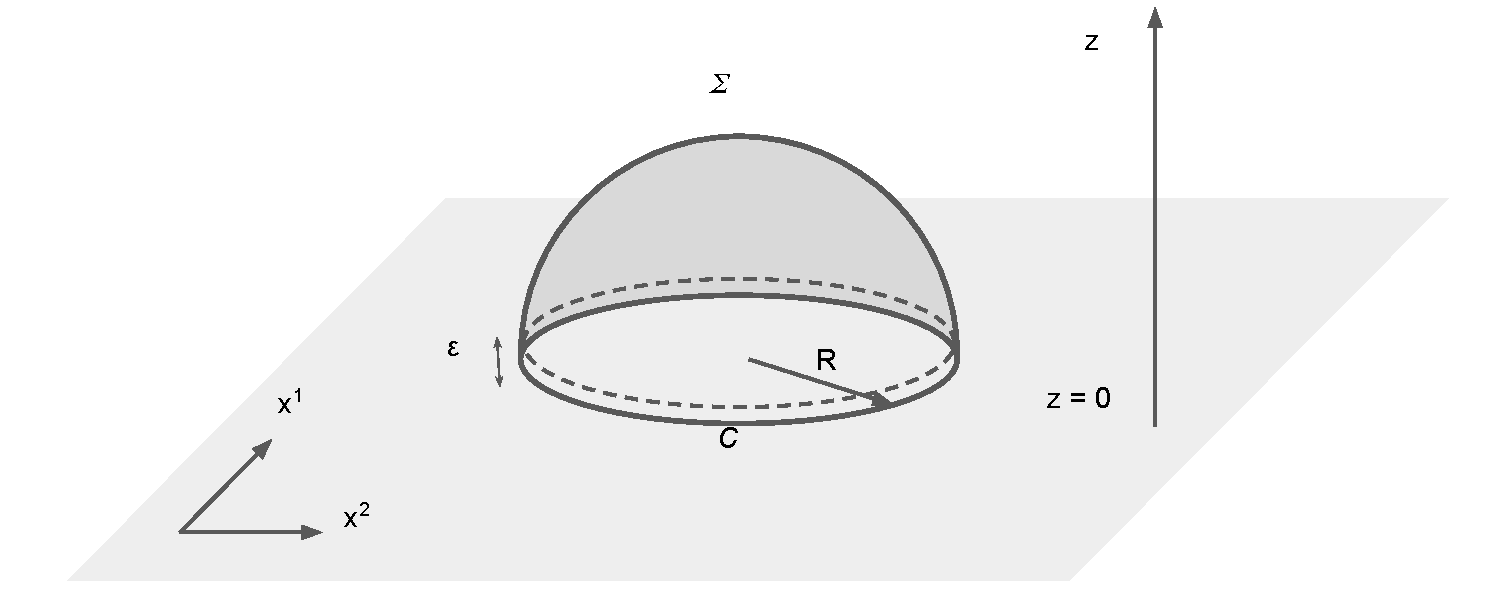
\includegraphics[width=11cm]{Images/WLcircle.pdf}
\end{center}
\caption{\label{fig:WLcircle} Circular Wilson loop as the minimal worldsheet area $\Sigma$ drawn by string ending in the contour $C$ at the boundary of $AdS_5$. }
\end{figure}

In the 't Hooft limit, which corresponds to classical supergravity limit,
minimizing the bosonic string action is sufficient for the leading order, which is essentially the minimal worldsheet area.
% \begin{equation}
%   W(C) \sim e^{-\sqrt{\lambda} A}.
% \end{equation}
Nevertheless, the area is infinite in $AdS$, hence we must regularize it.
For example, the minimal surface that is dual to the circular Wilson loop in the fundamental representation
is parametrized as
\begin{equation}
 z(r)=\sqrt{R^2-r^2}, \quad r\in[0, R], \quad \phi\in[0, 2\pi].
\end{equation}
This result can be obtained either by minimizing the string Nambu-Goto action \cite{Drukker:1999zq},
% \begin{equation}
%  S_\text{NG} = \dfrac{\sqrt{\lambda}}{2\pi} \int d^2 \sigma e^{\Phi/2} \sqrt{\text{det}}
% \end{equation}
or by exploiting the conformal symmetry, i.e. 
mapping the special conformal transformation of the straight line solution \cite{Berenstein:1998ij}.
The induced worldsheet metric, that is the pullback of the background metric $g$ \eqref{metricAdS} in polar coordinates for some $x^i$,
is:
\begin{equation}
 ds^2 = \dfrac{L^2}{z^2}\left((1+z'^2) dr^2 + r^2 d\phi^2 \right).
\end{equation}
Then the on-shell (Nambu-Goto) action gives:
\begin{eqnarray}
 S &=& T_\text{F1} \int \sqrt{\text{det} P[g]}\\
   &=& \dfrac{\sqrt{\lambda}}{2\pi} \int_0^{2\pi} d\phi \int_{0}^{\sqrt{R^2-\epsilon^2}} dr \dfrac{r}{z^2} \sqrt{1+z'^2}\\
   &=& \sqrt{\lambda} \left(\dfrac{R}{\epsilon}-1 \right). \label{minimalAction}
\end{eqnarray}
The correct prescription to regularize the action is to set the boundary cut-off at $z=\epsilon$,
then, we remove the perimeter divergence \cite{Drukker:1999zq}. 
This regularization scheme will be used for other cases of Wilson loop dual computations.
The finite remnant in \eqref{minimalAction} matches with the leading order field theory result \eqref{W1holographic}, i.e.
\begin{equation}
 W_1 = e^{\sqrt{\lambda}}, 
 \quad (N\rightarrow \infty \quad \text{and} \quad \lambda \rightarrow \infty).
\end{equation}

In order to compute the subleading correction 
% $\sqrt{2/\pi}\:\lambda^{-3/4}$ 
in \eqref{W1holographic}, 
the fermionic contribution must be taken into account. 
The full string action to use would be the Green-Schwarz action.
Although it is not fully known in curved background,
its quadratic order is known \cite{Cvetic:1999zs}, which suffices for 1-loop corrections. 
Its quartic order was also derived in \cite{Wulff:2013kga}.
Many efforts have been put into finding the subleading correction  
\cite{Kruczenski:2008zk, Kristjansen:2012nz, Bergamin:2015vxa, Forini:2015bgo, Faraggi:2016ekd, Forini:2017whz}
but no full matching has been achieved.
The ambiguity in the path integral measure hindered this computation.
% A way to evade it was to use the ratio of Wilson loops, and then the matching was proved for the ratio when expanding for small angles \cite{Forini:2017whz}.

\subsection{Higher rank representations}

The lesson from the fundamental Wilson loop suggests that 
the string dual of rank-$k$ representations must be an object that carries $k$ units of the string charge.
Intuitively, if we consider a Wilson loop wrapped $k$ times around the contour (the $k$-fundamental representation), 
we would expect the worldsheet to puff up, due to repulsive charges from multiple coincident fundamental strings.
We see that the individual string action is no longer useful in this case. 
Instead, we can describe the new object in terms of D-branes with fundamental string charges dissolve in it. 
% The charges are the source of a worldvolume electric field in the DBI action (ref).
The worldvolume must also pinch off at the boundary of $AdS_5$, 
ending along the curve defined by the Wilson loop, see figure \ref{fig:WLcircle}.
Supersymmetry will then guide us which D-brane configurations are allowed.


\begin{figure}[t]
\begin{center}
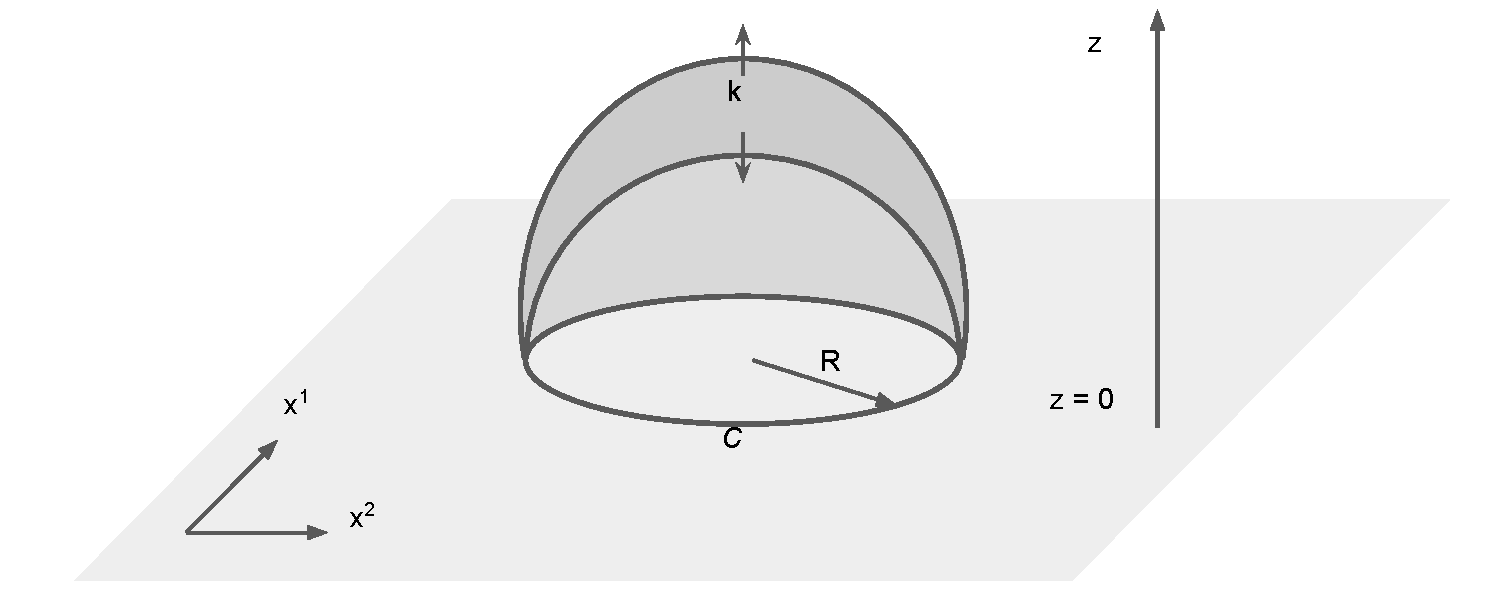
\includegraphics[width=11cm]{Images/DbraneWL.pdf}
\end{center}
\caption{\label{fig:DbraneWL} Circular Wilson loop of rank $k$ as a D-brane with $k$ string charges dissolved in it and the worldvolume ends in the contour $C$ at the boundary of $AdS_5$. }
\end{figure}


More generally, \cite{Gomis:2006sb} related supersymmetric Wilson loops of any representation of the gauge group 
to a stack of bulk D3-branes or a stack of bulk D5-branes, see figure \ref{fig:YoungTable}.
They proved the correspondence by explicitly integrating out the physics on the D-branes, 
which results to a half-BPS Wilson loop insertion in the desired representation in the $\mathcal{N}=4$ SYM path integral.

\begin{figure}[t]
\begin{center}
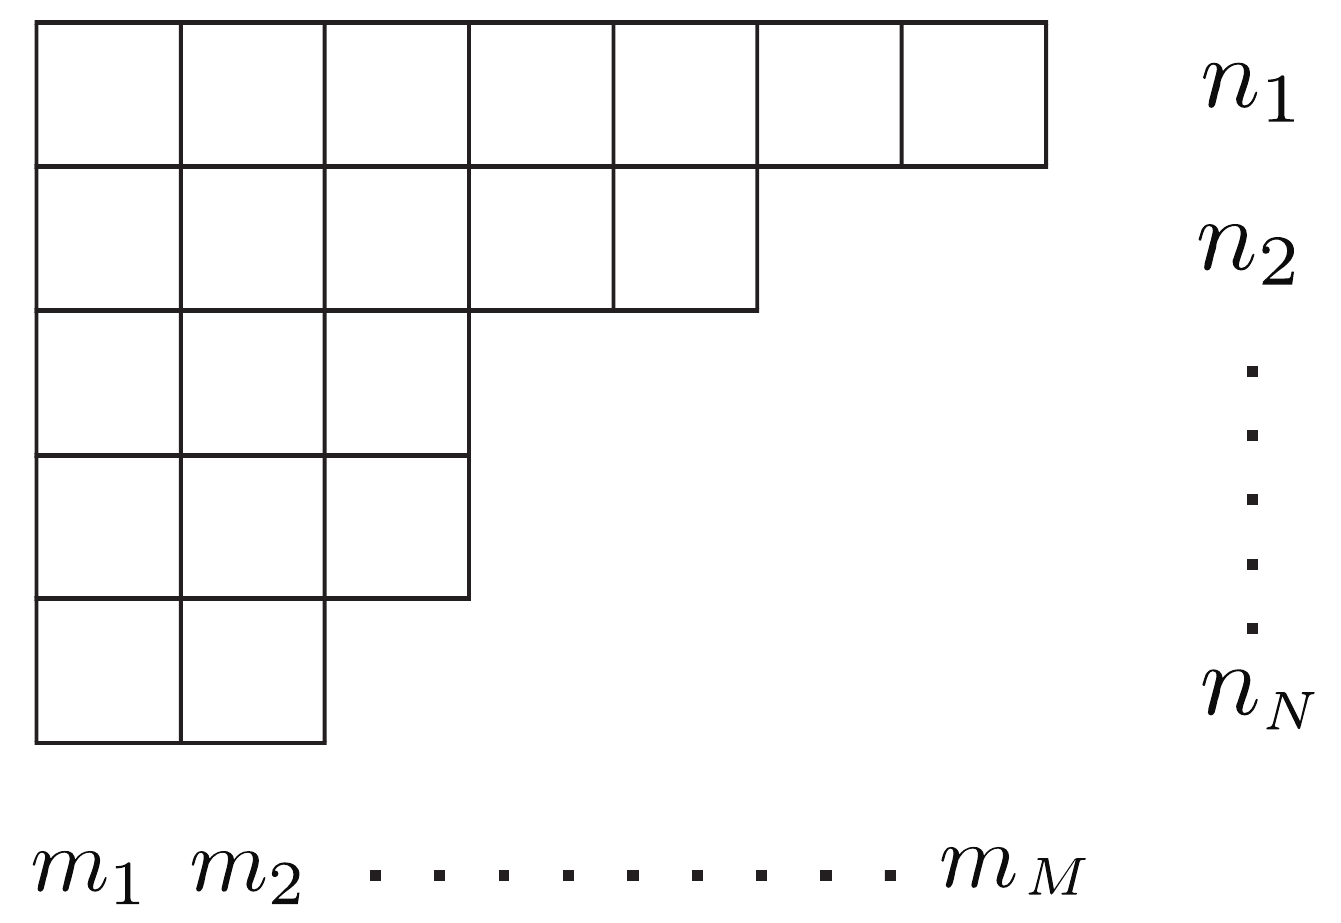
\includegraphics[width=7cm]{Images/YoungTable.png}
\end{center}
\caption{\label{fig:YoungTable} A generic Young table, taken from \cite{Gomis:2006sb}. 
Row $i$ corresponds to a D3-brane with $n_i$ fundamental string charge dissolved in it.
Column $j$ corresponds to a D5-brane with $m_j$ fundamental string charge dissolved in it.
Thus, for symmetric (one row) and antisymmetric (one column) representations,
their rank $k$ corresponds to the string charges a D3-brane and a D5-brane contains.}
\end{figure}

Let us focus on a single D3-brane and a single D5-brane.
Consider first the line element for $AdS_5\times S^5$ is this convenient form:
\begin{equation}
    ds^2 = L^2 \left( du^2 + \cosh^2 u \,d\check{\Omega}^2  + \sinh^2 u \, d\Omega_2^2 
  + d\theta^2 + \sin^2 \theta \, d\Omega_4^2 \right),
\end{equation}
where $u\geq 0$, and $\pi \geq \theta \geq 0 $. 
$d\check{\Omega}_n^2$ and $d\Omega_n^2$ indicate the line element for $AdS_n$ and $S^n$, respectively.
% and we use global coordinates to parametrize $AdS_2$ line element:
% \begin{equation}
%  d\check{\Omega}^2 =d\chi^2+\sinh^2\chi d\varphi^2, \quad \chi\geq 0, \quad 2 \pi \geq \varphi \geq 0.
% \end{equation}
Using the supersymmetry condition\footnote{
May be up to a sign depending on the conventions.}
\begin{equation}\label{susyCondition}
 \Gamma \epsilon =  \epsilon,
\end{equation}
where $\Gamma$ is the kappa symmetry\footnote{
It is a fermionic local gauge symmetry that is present also in particles and strings. 
Its full definition can be found in Paper III.}
projector for the D-brane and $\epsilon$ is the Killing spinor of the background geometry,
we can find the D-brane embeddings that preserve half of the original supersymmetries. 
Note that the supersymmetry condition, which gives first order differential equations,
imply the D-brane equations of motions, which are of second order, up to some integration constants. 
The list below shows the half-BPS D-brane embeddings with their worldvolume geometries
induced from the target space, and the worldvolume gauge fields $F$ \cite{Yamaguchi:2006tq}:
\begin{eqnarray}
 \text{D3-brane:} &\quad& AdS_2 \times S^2, \quad u=\text{constant}, \quad \theta = 0 \\
		  &\quad& \dfrac{1}{T_{F1}}F = L^2\sqrt{1+\kappa^2} e^0 e^1, \quad \kappa \equiv \sinh u \\
 \text{D5-brane:} &\quad& AdS_2 \times S^4, \quad u=0, \quad \theta = \text{constant} \\
 		  &\quad& \dfrac{1}{T_{F1}}F = L^2 \cos \theta e^0 e^1 
\end{eqnarray}
where $e^0$ and $e^1$ are the vielbeins\footnote{
Vielbeins are defined by $ds^2=\eta_{mn} e^m e^n$, which is often referred as the \emph{local frame}.
In terms of components: $e^m=e^m_M dx^M$, thus, we can relate them to the metric as $g_{MN} = \eta_{mn} e^m_M e^n_M$.} 
of $d\check{\Omega}^2$. 
We see that the D3-brane sits on a fixed point on the $S^5$, 
while the D5-brane sits on $S^4$ that is $\theta$ angle away from the pole of $S^5$, see figure \ref{fig:S5}.


\begin{figure}[t]
\begin{center}
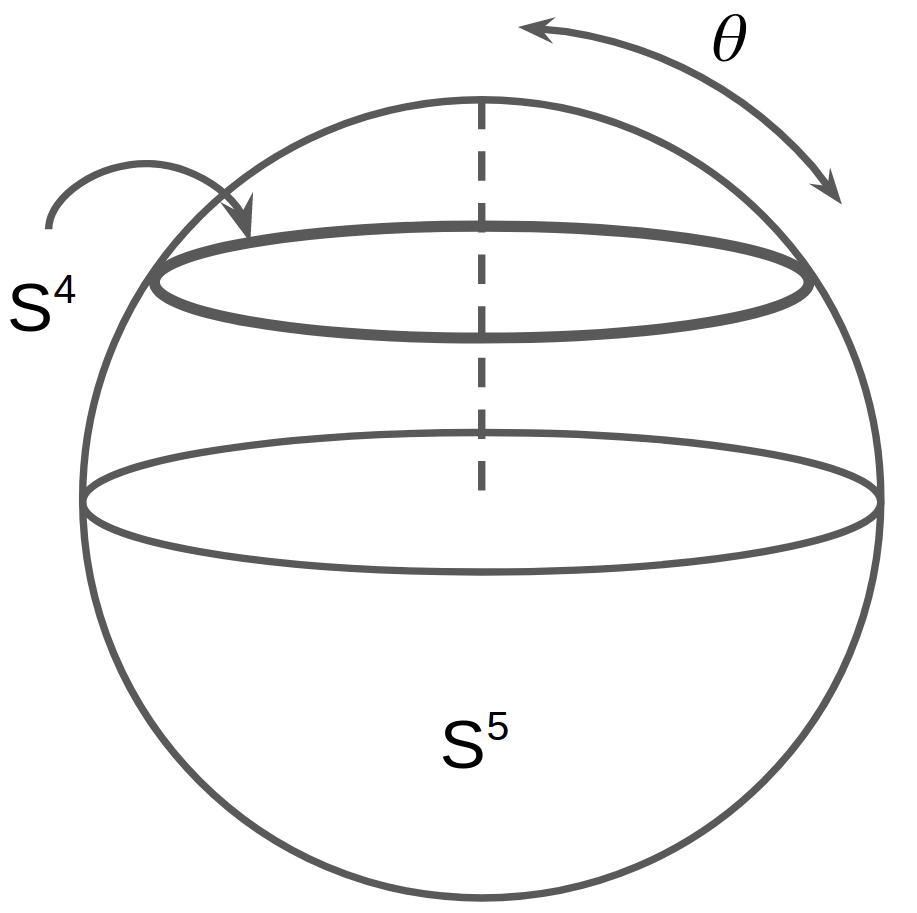
\includegraphics[width=4cm]{Images/S5.png}
\end{center}
\caption{\label{fig:S5} $S^4$ that is $\theta$ angle away from the pole of $S^5$. 
The angle depends on the amount of string charges $k$ that D5-brane contains.}
\end{figure}


The dual counterparts of the symmetric/antisymmetric representation in the leading order 't Hooft limit
are the on-shell action DBI \eqref{DBI} + WZ \eqref{WZ} of the D3-brane/D5-brane configuration aforementioned:
\begin{equation}\label{WLDbrane}
 \log W^{+}_k = - S_{D3}, \quad \log W^{-}_k = - S_{D5}.
\end{equation}
Moreover, we must ensure the string charge $k$ constraint, which can be added as a Lagrange multiplier term to the D-brane action:
\begin{equation} \label{stringChargeConstraint}
S_k = - k  \int_\Sigma F 
\quad \Rightarrow \quad  
k = \dfrac{1}{T_{F1}} \dfrac{\delta S_\text{DBI}}{\delta F} .
\end{equation}
The couplings in terms of $\lambda$ and $N$ are:
\begin{equation}
 T_\text{F1} = \dfrac{\sqrt{\lambda}}{2\pi L^2},
 \quad
%  T_\text{D1} = \dfrac{2N}{\sqrt{\lambda}},
%  \quad 
 T_\text{D3} = \dfrac{N}{2\pi^2 L^4},
 \quad 
 T_\text{D5} = \dfrac{N\sqrt{\lambda}}{8\pi^4 L^6},
\end{equation}
which are derived from \eqref{couplingsTension} using \eqref{couplings}.

Finally, the regularized actions are \cite{Drukker:2005kx, Yamaguchi:2006tq, Zarembo:2016bbk}: 
\begin{eqnarray}
 S_\text{D3} &=& - 2 N  (\kappa\sqrt{1+\kappa^2}+\mathop{\mathrm{arcsinh}}\kappa)\\
 S_\text{D5} &=& - N \frac{2\sqrt{\lambda }}{3\pi}\,\sin^3\theta,
\end{eqnarray}
with the $\theta$ satisfying the string charge constraint \eqref{stringChargeConstraint} that gives \eqref{eqThetaAntisym}, i.e. 
\begin{equation}
 \theta -\frac{1}{2}\,\sin 2\theta =\pi \frac{k}{N}.
\end{equation}
Thus the latitude angle $\theta$ depends on the amount of string charges $k$ dissolved in the D5-brane.
In conclusion, there is an exact agreement with \eqref{solW+} and \eqref{solW-}, according to \eqref{WLDbrane}.



\section{In Pilch-Warner background}

In $\mathcal{N}=2^*$ SYM on $S^4$, we took the decompactification limit for circular Wilson loops in order to have results on $\mathbb{R}^4$.
This means that in the Pilch-Warner background, the contour is a straight line of length $l\rightarrow \infty$. 

\subsection{Fundamental representation}
The minimal surface of a straight Wilson line is a wall,
with the worldsheet coordinates $(\tau, \sigma)$ induced from the Pilch-Warner geometry in the following way:
\begin{equation}
 \tau = x^1, \quad \sigma = c.
\end{equation}
The regularized on-shell action was computed in \cite{Buchel:2013id}, 
which agrees with the leading order result in \eqref{WLFundN2}, that is:
\begin{equation}\label{W1leading}
 \log W_1 = \sqrt{\lambda} M \frac{l}{2\pi }, \quad (l\rightarrow \infty).
\end{equation}


The goal of Paper V was to compute the loop corrections to the minimal surface 
by using string perturbation around the above classical solution.
There are two contributions, which turned out to be of equal weight in our case. 
The first one comes from the dilaton coupling to the worldsheet curvature called the Fradkin-Tseytlin term \cite{Fradkin:1983xs}:
\begin{equation}
 S_{FT}=\dfrac{1}{4\pi} \int d^2\sigma \sqrt{h}  R^{(2)} \Phi,
\end{equation}
which is actually a bit controversial, 
with some authors arguing it is not needed \cite{GRISARU1988625, GRISARU1985116, Cvetic:1999zs}.
Besides, it is zero for the familiar $AdS_5 \times S^5$ background due to a vanishing dilaton. 
% explicitly break the conformal invariance of the classical world-sheet action
The other one comes from 1-loop stringy corrections, 
which are computed by expanding the Green-Schwarz action up to quadratic fluctuations \cite{Cvetic:1999zs}.
These contribute as functional determinants, from generalizing the Gaussian integration formula \eqref{GaussianIntegral} for the bosons,
and the Grassmann integration for the fermions \eqref{GrassmannIntegral}.
Thus the semiclassical partition function is schematically of the form
\begin{equation}
 W = e^{-S_\text{cl}-S_\text{FT}} \dfrac{\text{det} F}{\sqrt{\text{det} B}},
\end{equation}
where $S_\text{cl}$ is the classical on-shell action in \eqref{W1leading}, 
$B$ and $F$ here just represent the bosonic and fermionic operators.
% of Schroedinger type (second order differential operator), 
% of Dirac type ($2\times2$ first order differential operator). 

Supersymmetry simplifies our problem by cancelling exactly 
the sector of bosonic and fermionic operators that are asymptotically massless (far away from the boundary $\sigma=1$).
The remaining sector is asymptotically massive, and the operators (after several manipulations) look enticingly similar:
\begin{equation}\label{basicDirac}
 H_B=\begin{pmatrix}
  1+\frac{A}{\sigma }  & \mathcal{L} \\ 
  \mathcal{L}^\dagger  & -1 \\ 
 \end{pmatrix},\qquad 
  H_F=\begin{pmatrix}
  -1                   & \mathcal{L} \\ 
  \mathcal{L}^\dagger  & 1+\frac{A}{\sigma }  \\ 
 \end{pmatrix},
\end{equation}
with
\begin{eqnarray}\label{EuclideanLs}
 \mathcal{L}&=&A\sqrt{\sigma ^2-1}\,\partial _\sigma +\frac{A\left(2\sigma ^2+1\right)}{2\sigma \sqrt{\sigma ^2-1}} ,
\nonumber \\
 \mathcal{L}^\dagger &=&-A\sqrt{\sigma ^2-1}\,\partial _\sigma 
-\frac{A\left(4\sigma ^2-1\right)}{2\sigma \sqrt{\sigma ^2-1}}
+\frac{2}{\sqrt{\sigma ^2-1}}\,.
\end{eqnarray}
The final semiclassical partition function to compute is then:
\begin{equation}\label{semiclassicalW}
  W = e^{-S_\text{cl}-S_\text{FT}}\dfrac{\text{det}^2 (\partial_\tau-H_F)}{\text{det}^2 (\partial_\tau-H_B)},
\end{equation}


Instead of using the heat kernel technique or the Gelfand-Yaglom method, 
both commonly used in the computation of functional determinants,
we used the phase-shift method from quantum mechanical scattering problems, see e.g. \cite{PhysRevD.10.4130}.
The method requires the operators to be asymptotically free, hence it works for (semi-)infinite intervals.
Our operators \eqref{basicDirac} share the same asymptotics in large $\sigma$, and they are defined in a semi-infinite interval $\sigma>1$,
so the method applies. Note that for $\tau$ variable, we do a usual Fourier transformation. 
The exponential of the ratio of the determinants of the operators in \eqref{semiclassicalW}
can be written in terms of the phase-shift $\delta(p)$ between the wave function and the asymptotic plane wave, 
see figure \ref{fig:potentialWavesPlot},
which is
\begin{equation}\label{deltaphases}    
 -2 \, \int_{0}^{\infty }\frac{dp}{2\pi }\,\,
 \frac{4 p }{9\sqrt{\frac{4}{9}\,p^2+1}}\,\left(
 \delta_F ^+(p)
 +
\delta_F ^-(p)
-\delta_B ^+(p)
 -
\delta_B^-(p)
\right) = -\dfrac{1}{4},
\end{equation}
where $\pm$ distinguish the two eigenvectors (particles and holes) of the Dirac Hamiltonians \eqref{basicDirac}.
The last equality is backed by our numerics.
Thus, together with the Fradkin-Tseytlin contribution, the total correction is $-1/2$. 
In conclusion, we do have a perfect matching with the field theory result \eqref{WLFundN2}.
% up to the subleading order in strong coupling expansion.
Moreover, the existence of Fradkin-Tseytlin term is necessary for this agreement.




\begin{figure}[t]
\begin{center}
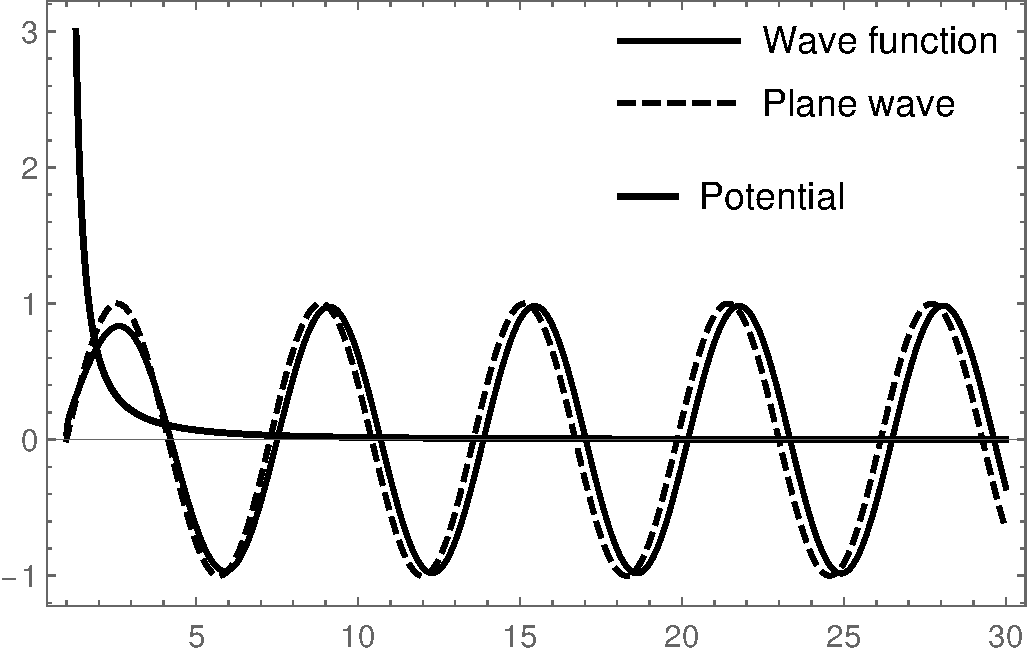
\includegraphics[width=0.7\textwidth]{Images/potentialWavesPlotBlack.pdf}
\end{center}
\caption{\label{fig:potentialWavesPlot} Phase-shift $\delta(p)$ of the wave function 
in the presence of a typical potential wall that many of our operators show, versus the free wave, 
for certain momentum $p$. 
}
\end{figure}


\subsection{Symmetric representation}
As for higher rank Wilson loops, Paper III found the D3-brane embedding dual to 
the straight Wilson line of length $l$ in symmetric representation, with the help of the supersymmetric condition \eqref{susyCondition}. 
The worldvolume metric is induced from the deformed $AdS$ part of \eqref{metricPW} in string frame\footnote{
We changed to mostly minus signature in order to follow Paper III.
The string metric $g$ and the Einstein metric $G$ are related by $g=e^{-\frac{4 \Phi }{D-2}} G$,
where $\Phi$ is the dilaton. 
}:
\begin{equation}
 ds^2 = \dfrac{A M^2 L^2}{c^2-1}\left(dx^2  - \rho(c)^2 d\Omega_2^2 \right)
	-L^2\left(\dfrac{1}{A \left(c^2-1\right)^2} + \dfrac{A M^2 \rho'(c)^2}{c^2-1} \right) dc^2,
\end{equation}
where 
\begin{equation}
 \rho(c)= \kappa \, \sqrt{c^2-1},
\end{equation}
since the deformed sphere shrinks to $\theta=\pi/2$ and $\phi=0$.
The worldvolume gauge field is given by
\begin{equation}
 \frac{1} {T_\text{F1}} F (c)  = -\dfrac{M L^2}{(c^2-1)^{3/2}} dx\wedge dc.
\end{equation}
As expected, it also reduces to the analogous case in $AdS_5 \times S^5$ close to the boundary. 

The regularized on-shell action reduces to
\begin{equation}
 S_{D3} = - \sqrt{\lambda} k M \dfrac{l}{2\pi}.
%  , \quad (l \rightarrow \infty).
\end{equation}
This agrees with the matrix model result \eqref{WsymPW} according to \eqref{WLDbrane}, only in the low rank limit
\begin{equation}
 \kappa \ll M l.
\end{equation}
Furthermore, for $k=1$, we recover the fundamental case \eqref{W1leading}.
We can conclude that this D3-brane configuration cannot probe the entire matrix model region, 
and a full dual object is still to be understood.

For the antisymmetric case, it is technically challenging to find the D5-brane solution. 
So far, we have not succeeded.
We do expect it though to match the leading order field theory result, 
because the matrix model result \eqref{WantisymPW} is proportional to $Ml$, the same as in the D-brane action.
It would be definitely interesting to compute the subleading order to determine the phase-transitions observed. 



     
   \chapter{Conclusions}



In this thesis, 
we explored a very special class of supersymmetric gauge theories whose path integrals are directly reducible to finite-dimensional integrals, 
i.e. 0-dimensional matrix models, by the means of the supersymmetric localization method.
In particular, we studied the vacuum partition function and the expectation values of BPS Wilson loop observables of $\mathcal{N}=2^*$ SYM on $S^4$.


Our main motivation was to rigorously test the gauge/string duality conjecture 
in a slightly more generalized setting than the well-known case of $\mathcal{N}=4$  SYM and type IIB strings on $AdS_5 \times S^5$, 
by introducing a mass scale. 
The total access to the strong coupling phase of $\mathcal{N}=2^*$ SYM gives us a golden opportunity to explicitly test it 
against its presumed dual theory of type IIB strings on the Pilch-Warner background.

Computations are highly non-trivial, 
on the gauge theory side, 
as well as on the string theory side. 
From our work, we can conclude the following, supplemented with possible future work:
\begin{itemize}
 \item Paper I and \cite{Zarembo:2014ooa} showed that the decompactifaction limit of $\mathcal{N}=2^*$ SYM on $S^4$ 
 commutes with the strong coupling limit. 
 This allows us to do holographic studies, 
 since the dual of $\mathcal{N}=2^*$ SYM on $\mathbb{R}^4$ is known. 
 For the sake of completeness, it would be interesting to extend the holographic study for the theory on $S^4$.
 
 \item 
%  There are infinitely-many phase transitions previously seen for finite critical couplings at the decompactification limit \cite{Russo:2013qaa}. 
 We used BPS Wilson loops in symmetric and antisymmetric representations of the gauge group to probe the strong-coupling phase of $\mathcal{N}=2^*$ SYM on $S^4$,
 especially in the decompactifaction limit, where infinite cusps appear.
 Paper II showed that these cusps induce phase transitions seen in the subleading order in strong coupling for these Wilson loops.
 In order to understand the nature of these phase transitions in the string theory side, 
 Paper III computed the D3-brane configuration in the Pilch-Warner background dual to the symmetric Wilson loop. 
 Only the leading result was derived, and it does not probe the full field theory result regime.
%  A different dual interpretation is needed to fully probe the field theory side solution though. 
%  Therefore, we have not been able to answer the question of the nature of the holographic description of the phase transitions. 
 From scaling arguments, we believe the D5-brane dual to the antisymmetric representation can be a promising case 
 for a full matching, and hopefully even at 1-loop level, where phase transitions happen. 
%  Unfortunately, due to technical difficulties, the solution has been elusive, 
% 
%  An attempt of a computer algebra program has been used to systematically solve the supersymmetric equations, 
%  and a new unpublished D7 brane solution has been found.
 
 
 \item The gauge/string duality for $\mathcal{N}=2^*$ case works with the fundamental Wilson line at least up to 1-loop quantum corrections, 
 shown numerically by Paper V. Given the simplicity of the field theory prediction, 
 an analytical result in the string theory side might be possible and desirable. 
 Moreover, the matching requires the existence of the controversial Fradkin-Tseytlin term in the string action. 
 It would be clarifying to prove its existence independently, for example by requiring the beta function of the Green-Schwarz action to be zero.
 
  \item It is known that Wilson loops in the symmetric representation and the multiply-wrapped representation differ 
 by exponentially suppressed terms for strong coupling \cite{Yamaguchi:2007ps}. 
 Paper IV provided a non-planar correction to this statement for the $\mathcal{N}=4$ case, 
 and helped to clarify a mismatch in an open problem concerning 1-loop corrections 
 in the holographic dual computation \cite{Faraggi:2014tna, Buchbinder:2014nia}. 
 Solving this problem is definitely a further non-trivial quantum rigorous test, 
 and we would gain a better understanding of divergences in stringy corrections. 
 There is a similar open problem concerning 1-loop matching for circular fundamental Wilson loop 
 in $\mathcal{N}=4$ SYM \cite{Kruczenski:2008zk, Kristjansen:2012nz, Bergamin:2015vxa, Forini:2015bgo, Faraggi:2016ekd, Forini:2017whz}.
%  \item 

\end{itemize}


Despite technical challenges, 
further studies on this $\mathcal{N}=2^*$SYM case are necessary for better rigorous understanding of the generic gauge/string duality.


  
   \chapter{Sammanfattning}



Gauge/str\"ang-dualiteten (eller den holografiska principen) \"ar en anm\"arkningsv\"ard och djup f\"ormodan som kommer fr\r{a}n str\"angteorins m\r{a}ngfasetterade ramverket. Den relaterar starkt kopplade gaugeteorier till svagt kopplad str\"angteori i en h\"ogre-dimensionell kr\"okt geometri. Fr\r{a}n en konceptuell synvinkel antyder den att gravitation, vilken \"ar str\"angteorins l\r{a}genergigr\"ans, och s\r{a}lunda rumtiden, \"ar ett emergent fenomen fr\r{a}n en l\"agre-dimensionell gaugeteori. Fr\r{a}n en praktisk synvinkel m\"ojligg\"or dualiteten att familj\"ara verktyg inom gravitationsteorier kan ge svar till beryktat sv\r{a}ra fr\r{a}gest\"allningar inom gaugeteori vid stark koppling. Eftersom att gaugeteorier \"ar s\r{a} vanligt f\"orekommande inom fysik -- fr\r{a}n beskrivningen av fundamentala interaktioner i partikelfysik till modellering av kondenserad materia-system -- \"ar ett s\r{a}dant analytiskt verktyg potentiellt v\"aldigt lovande. Exempel p\r{a} \"annu ol\"osta problem som skulle kunna l\"osas genom dualiteten \"ar confinement i kvantkromodynamik, eller att f\"orst\r{a} faserna i en okonventionell supraledare.
 
 
Brasklappen hos denna "f\"or-bra-f\"or-att-vara-sann"-dualitet \"ar att v\"aldigt lite \"ar k\"ant om den, f\"orutom i vissa specialfall. Den b\"ast f\"orst\r{a}dda versionen \"ar AdS/CFT-korrespondensen, vilken h\"avdar att $\mathcal{N}=4$ SYM, som \"ar en gaugeteori med supersymmetri och konform symmetri, \"ar ekvivalent med typ IIB sluten str\"angteori i en 10-dimensionell $AdS_5 \times S^5$-bakgrund. Under de senaste 20 \r{a}ren sedan Maldacena f\"orst formulerade detta antagande har m\r{a}nga rigor\"osa tester utf\"orts. F\r{a} experter inom f\"altet, om n\r{a}gon, betvivlar numer riktigheten av just denna korrespondens.  Denna framg\r{a}ng inspirerar till generaliseringar till mindre symmetriska teorier. N\"ar allt kommer omkring s\r{a} \"ar $\mathcal{N}=4$ SYM s\r{a} begr\"ansad av sina symmetrier att det \"ar troligt att den \"ar tillfullo kvantintegrabel.
 
 
N\"asta naturliga steg \"ar att l\"agga till massiva tillst\r{a}nd till $\mathcal{N}=4$ SYM. Den unika massdeformation vilken bevarar h\"alften av supersymmetrin men bryter den konforma symmetrin \"ar den s\r{a} kallade $\mathcal{N}=2^*$ SYM. Det \"ar denna teori som \"ar studie\"amnet f\"or denna avhandling. Den \"ar tillr\"ackligt supersymmetrisk f\"or att den kraftfulla metoden supersymmetrisk lokalisering skall kunna anv\"andas, genom vilken $\mathcal{N}=2^*$-teorins partitionsfunktion \"over en sf\"ar reduceras till en effektiv matrismodell. P\r{a} s\r{a} vis \"ar ber\"akningskomplexiteten kraftigt reducerad s\r{a} att standardmetoder f\"or slumpm\"assiga matriser kan anv\"andas. \r{A} andra sidan orsakar de introducerade masskalorna icke-triviala fasstrukturer i vakuumf\"altkonfigurationerna, i gr\"ansen av platt rum. Detta saknar uppenbarligen motstycke i fallet med $\mathcal{N}=4$ SYM d\r{a} den senare \"ar massl\"os. Att f\"orst\r{a} denna nya egenskap, b\r{a}de inom f\"altteorin och framf\"or allt i den duala gravitationsteorin, \"ar ett av avhandlingens huvudmotiv.
 
Gravitationsdualen till $\mathcal{N}=2^*$ SYM utan kr\"okning \"ar den s\r{a} kallade Pilch-Warner-bakgrunden. Denna geometri \"ar en deformerad $AdS_5 \times S^5$, och den reduceras asymptotiskt till den senare n\"ara den konforma randen. Alla supergravitationsf\"alt \"ar icke-triviala, till skillnad fr\r{a}n den enklaste situationen i $AdS_5 \times S^5$-bakgrunden. Tyv\"arr f\"orsv\r{a}rar detta ber\"akningar betydligt. Icke desto mindre har vi lyckats att rigor\"ost och framg\r{a}ngsrikt testa denna icke-konforma version av AdS/CFT-korrespondensen f\"or vissa observabler.
 
Observablerna som vi studerar \"ar supersymmetriska Wilson-loopar i olika representationer av gaugegruppen. F\"or den fundamentala Wilson-loopen, dual till str\"angdiskpartitionfunktionen, lyckades vi med \"overensst\"ammelse j\"amf\"ora f\"altteorif\"oruts\"agelsen genom att ber\"akna str\"angkorrektionerna till den minimala arean. Detta \"ar det f\"orsta testet p\r{a} kvantniv\r{a} som har gjorts i denna icke-konforma s\"attning. \r{A} andra sidan bevisade vi att Wilson-loopar med representationer av h\"ogre rang uppvisar de fas\"overg\r{a}ngarna som observerats i vakuumpartitionsfunktionen vid andra ordningens stark koppling. Deras duala objekt \"ar supersymmetriska, elektriskt laddade D-bran. Vi lyckades finna D-branskonfigurationen som \"ar dual till Wilson loopen i den symmetriska representationen och visade att korrespondensen h\r{a}ller till f\"orsta ordningen, \r{a}tminstone i en specifik gr\"ans av det f\"altteoretiska resultatet. Loopkorrektionerna kan d\"armed inte ha de n\"amnda fas\"overg\r{a}ngarna. Det senare kvarst\r{a}r som ett \"oppet problem och vi f\"orv\"antar oss fortsatt arbete kring den anti-symmetriska representationens D-branskonfiguration f\"or att vidare belysa detta.

  
   \chapter{Acknowledgement}


First of all, I would like to thank Kostya for being my supervisor, teacher and a model physicist. 
Much of the success of this thesis is due to him, as well as to the hard-work and perseverance of my other collaborators: Amit, Daniel and Jamie. I very much appreciate having you to discuss our projects and work together.

I also thank Kostya and Amit for proofreading parts of my manuscript. Thanks goes to Erik for the Swedish translation of the summary. 

I thank Nordita for a nice working environment, and fellow students Erik, Daniel and Janina, who literally added light, music and chocolate to the office.

I would like to thank the GATIS network for funding my first three years of research and training my soft skills.

Last but not least, let me finally acknowledge my dearest Stephane, for his more-than-a-thousand times speedup of the numerical code used in my first paper, and his careful proofreading of many of my texts, including parts of this thesis.  
      
	
\backmatter
    % References
    % No restriction is set to the reference styles
    % Save your references in References.bib
%     \nocite{*} % Remove this for your own citations
    \bibliographystyle{utphys} %halpha has no hyperlink!
    \bibliography{References}


\end{document}\grid
\grid
\grid
\grid
\grid
\grid
